\documentclass[]{article}
\usepackage{lmodern}
\usepackage[compact]{titlesec}
\usepackage{amssymb,amsmath}
\usepackage{ifxetex,ifluatex}
\usepackage{fixltx2e} % provides \textsubscript
\ifnum 0\ifxetex 1\fi\ifluatex 1\fi=0 % if pdftex
  \usepackage[T1]{fontenc}
  \usepackage[utf8]{inputenc}
\else % if luatex or xelatex
  \ifxetex
    \usepackage{mathspec}
  \else
    \usepackage{fontspec}
  \fi
  \defaultfontfeatures{Ligatures=TeX,Scale=MatchLowercase}
\fi
% use upquote if available, for straight quotes in verbatim environments
\IfFileExists{upquote.sty}{\usepackage{upquote}}{}
% use microtype if available
\IfFileExists{microtype.sty}{%
\usepackage{microtype}
\UseMicrotypeSet[protrusion]{basicmath} % disable protrusion for tt fonts
}{}
\usepackage[margin=1in]{geometry}
\usepackage{hyperref}
\hypersetup{unicode=true,
            pdftitle={Assignment 3: Wine Sales Project},
            pdfauthor={Darryl Buswell},
            pdfborder={0 0 0},
            breaklinks=true}
\urlstyle{same}  % don't use monospace font for urls
\usepackage{color}
\usepackage{fancyvrb}
\newcommand{\VerbBar}{|}
\newcommand{\VERB}{\Verb[commandchars=\\\{\}]}
\DefineVerbatimEnvironment{Highlighting}{Verbatim}{commandchars=\\\{\}}
% Add ',fontsize=\small' for more characters per line
\usepackage{framed}
\definecolor{shadecolor}{RGB}{248,248,248}
\newenvironment{Shaded}{\begin{snugshade}}{\end{snugshade}}
\newcommand{\KeywordTok}[1]{\textcolor[rgb]{0.13,0.29,0.53}{\textbf{{#1}}}}
\newcommand{\DataTypeTok}[1]{\textcolor[rgb]{0.13,0.29,0.53}{{#1}}}
\newcommand{\DecValTok}[1]{\textcolor[rgb]{0.00,0.00,0.81}{{#1}}}
\newcommand{\BaseNTok}[1]{\textcolor[rgb]{0.00,0.00,0.81}{{#1}}}
\newcommand{\FloatTok}[1]{\textcolor[rgb]{0.00,0.00,0.81}{{#1}}}
\newcommand{\ConstantTok}[1]{\textcolor[rgb]{0.00,0.00,0.00}{{#1}}}
\newcommand{\CharTok}[1]{\textcolor[rgb]{0.31,0.60,0.02}{{#1}}}
\newcommand{\SpecialCharTok}[1]{\textcolor[rgb]{0.00,0.00,0.00}{{#1}}}
\newcommand{\StringTok}[1]{\textcolor[rgb]{0.31,0.60,0.02}{{#1}}}
\newcommand{\VerbatimStringTok}[1]{\textcolor[rgb]{0.31,0.60,0.02}{{#1}}}
\newcommand{\SpecialStringTok}[1]{\textcolor[rgb]{0.31,0.60,0.02}{{#1}}}
\newcommand{\ImportTok}[1]{{#1}}
\newcommand{\CommentTok}[1]{\textcolor[rgb]{0.56,0.35,0.01}{\textit{{#1}}}}
\newcommand{\DocumentationTok}[1]{\textcolor[rgb]{0.56,0.35,0.01}{\textbf{\textit{{#1}}}}}
\newcommand{\AnnotationTok}[1]{\textcolor[rgb]{0.56,0.35,0.01}{\textbf{\textit{{#1}}}}}
\newcommand{\CommentVarTok}[1]{\textcolor[rgb]{0.56,0.35,0.01}{\textbf{\textit{{#1}}}}}
\newcommand{\OtherTok}[1]{\textcolor[rgb]{0.56,0.35,0.01}{{#1}}}
\newcommand{\FunctionTok}[1]{\textcolor[rgb]{0.00,0.00,0.00}{{#1}}}
\newcommand{\VariableTok}[1]{\textcolor[rgb]{0.00,0.00,0.00}{{#1}}}
\newcommand{\ControlFlowTok}[1]{\textcolor[rgb]{0.13,0.29,0.53}{\textbf{{#1}}}}
\newcommand{\OperatorTok}[1]{\textcolor[rgb]{0.81,0.36,0.00}{\textbf{{#1}}}}
\newcommand{\BuiltInTok}[1]{{#1}}
\newcommand{\ExtensionTok}[1]{{#1}}
\newcommand{\PreprocessorTok}[1]{\textcolor[rgb]{0.56,0.35,0.01}{\textit{{#1}}}}
\newcommand{\AttributeTok}[1]{\textcolor[rgb]{0.77,0.63,0.00}{{#1}}}
\newcommand{\RegionMarkerTok}[1]{{#1}}
\newcommand{\InformationTok}[1]{\textcolor[rgb]{0.56,0.35,0.01}{\textbf{\textit{{#1}}}}}
\newcommand{\WarningTok}[1]{\textcolor[rgb]{0.56,0.35,0.01}{\textbf{\textit{{#1}}}}}
\newcommand{\AlertTok}[1]{\textcolor[rgb]{0.94,0.16,0.16}{{#1}}}
\newcommand{\ErrorTok}[1]{\textcolor[rgb]{0.64,0.00,0.00}{\textbf{{#1}}}}
\newcommand{\NormalTok}[1]{{#1}}
\usepackage{longtable,booktabs}
\usepackage{graphicx,grffile}
\makeatletter
\def\maxwidth{\ifdim\Gin@nat@width>\linewidth\linewidth\else\Gin@nat@width\fi}
\def\maxheight{\ifdim\Gin@nat@height>\textheight\textheight\else\Gin@nat@height\fi}
\makeatother
% Scale images if necessary, so that they will not overflow the page
% margins by default, and it is still possible to overwrite the defaults
% using explicit options in \includegraphics[width, height, ...]{}
\setkeys{Gin}{width=\maxwidth,height=\maxheight,keepaspectratio}
\IfFileExists{parskip.sty}{%
\usepackage{parskip}
}{% else
\setlength{\parindent}{0pt}
\setlength{\parskip}{6pt plus 2pt minus 1pt}
}
\setlength{\emergencystretch}{3em}  % prevent overfull lines
\providecommand{\tightlist}{%
  \setlength{\itemsep}{0pt}\setlength{\parskip}{0pt}}
\setcounter{secnumdepth}{0}
% Redefines (sub)paragraphs to behave more like sections
\ifx\paragraph\undefined\else
\let\oldparagraph\paragraph
\renewcommand{\paragraph}[1]{\oldparagraph{#1}\mbox{}}
\fi
\ifx\subparagraph\undefined\else
\let\oldsubparagraph\subparagraph
\renewcommand{\subparagraph}[1]{\oldsubparagraph{#1}\mbox{}}
\fi

%%% Use protect on footnotes to avoid problems with footnotes in titles
\let\rmarkdownfootnote\footnote%
\def\footnote{\protect\rmarkdownfootnote}

%%% Change title format to be more compact
\usepackage{titling}

% Create subtitle command for use in maketitle
\newcommand{\subtitle}[1]{
  \posttitle{
    \begin{center}\large#1\end{center}
    }
}

\setlength{\droptitle}{-2em}
  \title{Assignment 3: Wine Sales Project}
  \pretitle{\vspace{\droptitle}\centering\huge}
  \posttitle{\par}
\subtitle{MSPA PREDICT 411-DL-SEC56}
  \author{Darryl Buswell}
  \preauthor{\centering\large\emph}
  \postauthor{\par}
  \date{}
  \predate{}\postdate{}

\begin{document}
\maketitle

\section{1 Introduction}\label{introduction}

This document presents results of the third assignment for the Masters
of Science in Predictive Analytics course: PREDICT 411. This assessment
required the student to build predictive models which are able to
predict the number of wine cases ordered by wine distribution companies.
To achieve this, we built five predictive models, including a linear
regression model and four generalized linear regression models. Each
were specified using automated variable selection techniques. As a final
step for this assessment, we present a SAS routine which is able to
generate predictions of wine orders based on a withheld test set of
data.

\section{2 Data}\label{data}

The dataset contains 12,000 data records, with variables which
characterize commercially available wines. The variables are mostly
related to the chemical properties of the wine being sold. The target
variable is the number of sample cases of wine that were purchased by
wine distribution companies after they had sampled the wine. At a first
pass, it seems the dataset has quite a large amount of scope. There are
14 variables tracking a number of attributes. The table below shows a
list of variables included in the original dataset.

\paragraph{Table 2.1: Variable
Descriptions}\label{table-2.1-variable-descriptions}

\begin{longtable}[]{@{}lll@{}}
\toprule
Original Variable & Renamed Variable & Description\tabularnewline
\midrule
\endhead
AcidIndex & N\_AcidIndex & Method of testing total acidity of
wine\tabularnewline
Alcohol & N\_Alcohol & Alcohol Content\tabularnewline
Chlorides & N\_Chlorides & Chloride content of wine\tabularnewline
CitricAcid & N\_CitricAcid & Citric Acid Content\tabularnewline
Density & N\_Density & Density of Wine\tabularnewline
FixedAcidity & N\_FixedAcidity & Fixed Acidity of Wine\tabularnewline
FreeSulfurDioxide & N\_FreSulfDiox & Sulfur Dioxide content of
wine\tabularnewline
LabelAppeal & N\_LabelAppeal & Marketing Score indicating the appeal of
label\tabularnewline
ResidualSugar & N\_ResSugar & Residual Sugar of wine\tabularnewline
STARS & N\_STARS & Wine rating by a team of experts\tabularnewline
Sulphates & N\_Sulphates & Sulfate content of wine\tabularnewline
TotalSulfurDioxide & N\_TotSulfDiox & Total Sulfur Dioxide of
Wine\tabularnewline
VolatileAcidity & N\_VolAcid & Volatile Acid content of
wine\tabularnewline
pH & N\_pH & pH of wine\tabularnewline
\bottomrule
\end{longtable}

For this assessment, we have renamed each variable according to its
format type. Since all variables are of numeric type, each have been
renamed to include a `N\_' prefix.

\section{3 Data Exploration}\label{data-exploration}

Prior to performing any model building, a number of data exploration
routines were conducted. These routines allow us to gain an
understanding of any potential limitations of the dataset including
identifying variables which have missing observations, outlier
observations, or those variables which may benefit from transformation.

\subsection{3.1 Univariate Data
Analysis}\label{univariate-data-analysis}

Summary statistics for each of the numeric variables is shown in the
table below.

\paragraph{Table 3.1.1: Data
Statistics}\label{table-3.1.1-data-statistics}

\begin{longtable}[]{@{}lllllll@{}}
\toprule
Variable & Minimum & Maximum & Mean & Std Dev & N Miss &
N\tabularnewline
\midrule
\endhead
N\_FixedAcidity & -18.1 & 34.4 & 7.0757171 & 6.3176435 & 0 &
12795\tabularnewline
N\_VolAcid & -2.79 & 3.68 & 0.3241039 & 0.7840142 & 0 &
12795\tabularnewline
N\_CitricAcid & -3.24 & 3.86 & 0.3084127 & 0.8620798 & 0 &
12795\tabularnewline
N\_ResSugar & -127.8 & 141.15 & 5.4187331 & 33.749379 & 616 &
12179\tabularnewline
N\_Chlorides & -1.171 & 1.351 & 0.0548225 & 0.3184673 & 638 &
12157\tabularnewline
N\_FreSulfDiox & -555 & 623 & 30.8455713 & 148.7145577 & 647 &
12148\tabularnewline
N\_TotSulfDiox & -823 & 1057 & 120.7142326 & 231.9132105 & 682 &
12113\tabularnewline
N\_Density & 0.88809 & 1.09924 & 0.9942027 & 0.0265376 & 0 &
12795\tabularnewline
N\_pH & 0.48 & 6.13 & 3.2076282 & 0.6796871 & 395 & 12400\tabularnewline
N\_Sulphates & -3.13 & 4.24 & 0.5271118 & 0.9321293 & 1210 &
11585\tabularnewline
N\_Alcohol & -4.7 & 26.5 & 10.4892363 & 3.727819 & 653 &
12142\tabularnewline
N\_LabelAppeal & -2 & 2 & -0.009066 & 0.8910892 & 0 &
12795\tabularnewline
N\_AcidIndex & 4 & 17 & 7.7727237 & 1.3239264 & 0 & 12795\tabularnewline
N\_STARS & 1 & 4 & 2.041755 & 0.90254 & 3359 & 9436\tabularnewline
\bottomrule
\end{longtable}

First, we can see that a number of variables suffer from missing
observations and will therefore benefit from some form of imputation.
In-fact only six variables were found to not include missing
observations. Second, we note a number of inconsistencies in the data.
For example, wine cannot have a negative alcohol content, indicating
that the minimum value of -4.7 is erroneous (Robinson 2006). Similarly,
the minimum residual sugar (-127.8 g/L) is implausible as wines
typically have a sugar content greater than 1 g/L (Peynaud 1987). Third,
we note that a comparison of the minimum/maximum versus standard
deviation value suggests the existence of outliers for a number of
variables.

We also looked to compare the mean and variance of the target variable
in an attempt to check for the assumption of equality for the Poisson or
Negative Binomial distribution. We found the target mean value (3.03) to
be quite similar to its variance (3.71), which suggests that we would be
in violation of the assumption of equal mean and variance for the
Poisson distribution, but not in violation of the assumption that the
variance be larger than the mean for the Negative Binomial distribution.

Visualization methods can also be used to gain a greater understanding
of each variable. For this assessment, histogram and box plots were
generated and reviewed for all numeric variables. We have selected a
number of variables for further discussion below.

\newpage

\paragraph{Figure 3.1.1 Histogram:
Density}\label{figure-3.1.1-histogram-density}

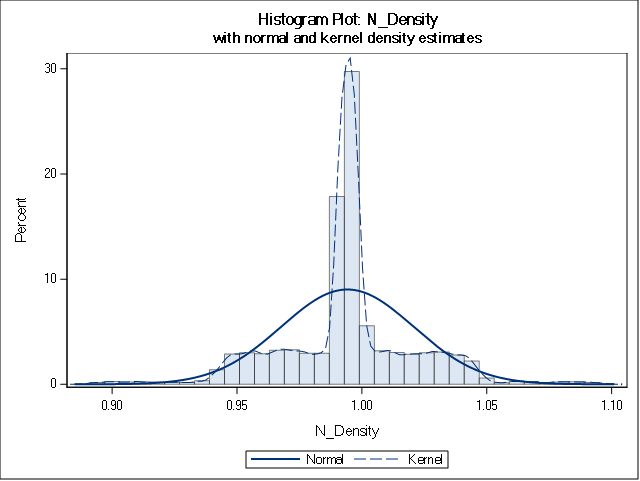
\includegraphics[height=3.95833in]{images/hist_density.png}

\paragraph{Figure 3.1.2 Box Plot:
Density}\label{figure-3.1.2-box-plot-density}

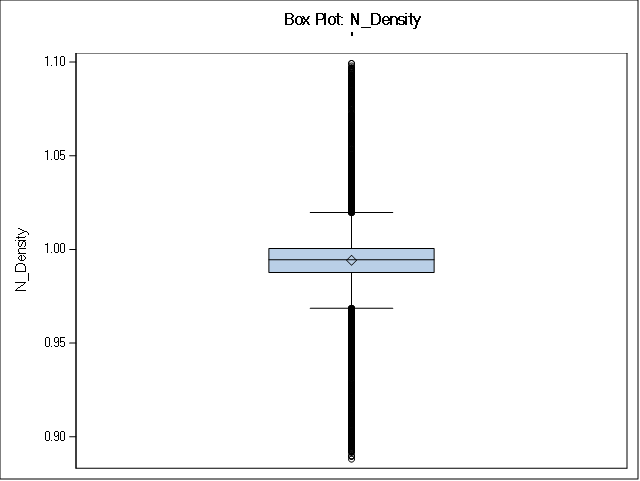
\includegraphics[height=3.95833in]{images/box_density.png}

\newpage

\paragraph{Figure 3.1.3 Histogram: Acid
Index}\label{figure-3.1.3-histogram-acid-index}

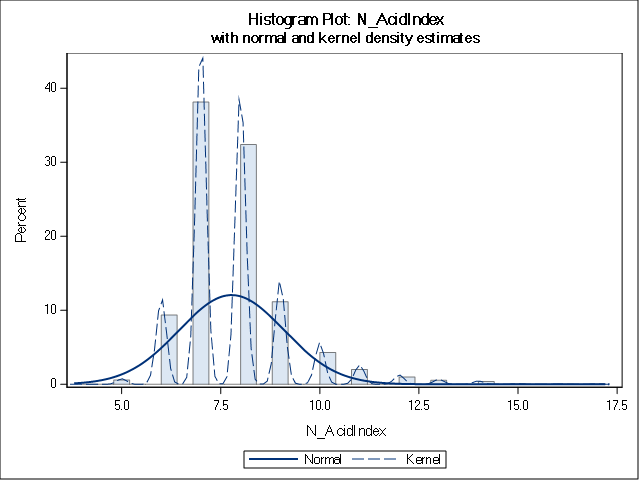
\includegraphics[height=3.95833in]{images/hist_acidindex.png}

\paragraph{Figure 3.1.4 Box Plot: Acid
Index}\label{figure-3.1.4-box-plot-acid-index}

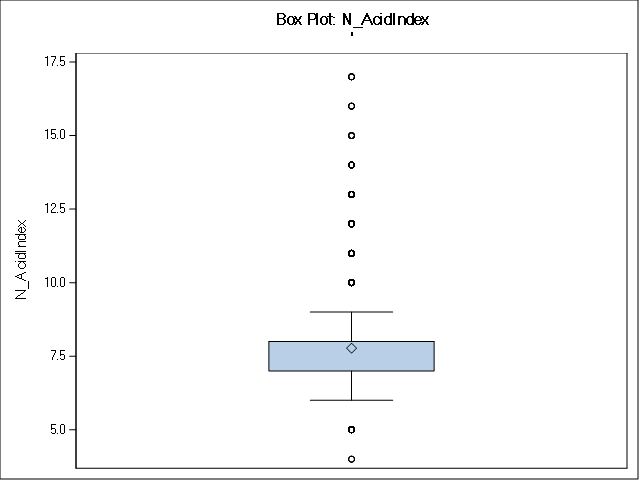
\includegraphics[height=3.95833in]{images/box_acidindex.png}

\newpage

Many variables share the same characteristics as density (N\_Density).
That is, a tight collection of observations around the mean and fat
tails, suggesting a high amount of kurtosis. Chlorides (N\_Chlorides) in
particular seems to have the highest amount of kurtosis of each
variable. This quality makes outlier identification difficult, as can be
seen by the box plot for density above.

There are also some examples of variables which are non-continuous in
nature. Acid index (N\_AcidIndex) and the appeal label (N\_LabelAppeal)
for example have their observations binned over certain values. We note
that this is also the case for the target variable, which does seem to
be normally distributed, however its non-continuous nature and amount of
zero observations will cause issues when fitting standard Ordinary Least
Square (OLS) based models.

\subsection{3.2 Bivariate Data Analysis}\label{bivariate-data-analysis}

Since we intend on building a prediction model for the number of
purchased cases of wine, we have an interest in those variables which
have explanatory power over this variable. As such, we first check the
Pearson correlation coefficient in relation between each numeric
variable and our target.

The table below summarizes the correlation coefficients between our
target and each numeric variable.

\paragraph{Table 3.2.1: Correlations for Purchased Cases vs.~Numeric
Data}\label{table-3.2.1-correlations-for-purchased-cases-vs.numeric-data}

\begin{longtable}[]{@{}ll@{}}
\toprule
Variable & Correlation\tabularnewline
\midrule
\endhead
N\_FixedAcidity & -0.04901\tabularnewline
N\_VolAcid & -0.08879\tabularnewline
N\_CitricAcid & 0.00868\tabularnewline
N\_ResSugar & 0.01649\tabularnewline
N\_Chlorides & -0.03826\tabularnewline
N\_FreSulfDiox & 0.04382\tabularnewline
N\_TotSulfDiox & 0.05148\tabularnewline
N\_Density & -0.03552\tabularnewline
N\_pH & -0.00944\tabularnewline
N\_Sulphates & -0.03885\tabularnewline
N\_Alcohol & 0.06206\tabularnewline
N\_LabelAppeal & 0.3565\tabularnewline
N\_AcidIndex & -0.24605\tabularnewline
N\_STARS & 0.55879\tabularnewline
\bottomrule
\end{longtable}

None of the numeric variables are reported to have a strong positive or
negative correlation coefficient with the response variable, with the
greatest absolute correlation being reported by wine rating (N\_STARS)
and appeal label (N\_LabelAppeal) at 0.56 and 0.36 respectively.
However, it is well established that wine taste is determined by the
level of sugar. alcohol, acids and tannins in the beverage (Robinson
2006). This may indicate that a diverse range of wines appealed to the
wine tasters and/or their preferences may have been influenced by
factors other than taste.

We can also use scatter plots with a Locally Estimated Scatter Plot
Smoother (LOESS) overlay to further explore the relationship between the
target and each predictor variable. Scatter plots for a collection of
variables against the response variable were generated and reviewed with
two of these plots selected for further discussion below.

\newpage

\paragraph{Figure 3.2.1 Scatter: Purchased Cases
vs.~Density}\label{figure-3.2.1-scatter-purchased-cases-vs.density}

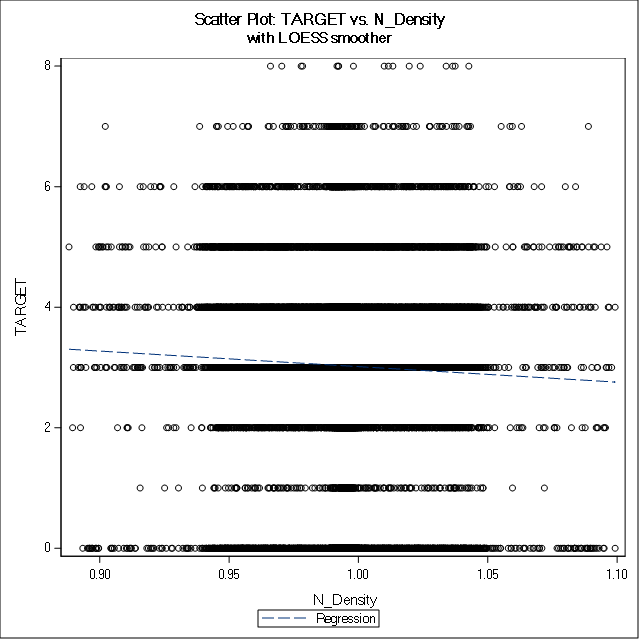
\includegraphics[height=3.95833in]{images/scatter_density.png}

\paragraph{Figure 3.2.2 Scatter: Purchased Cases
vs.~Stars}\label{figure-3.2.2-scatter-purchased-cases-vs.stars}

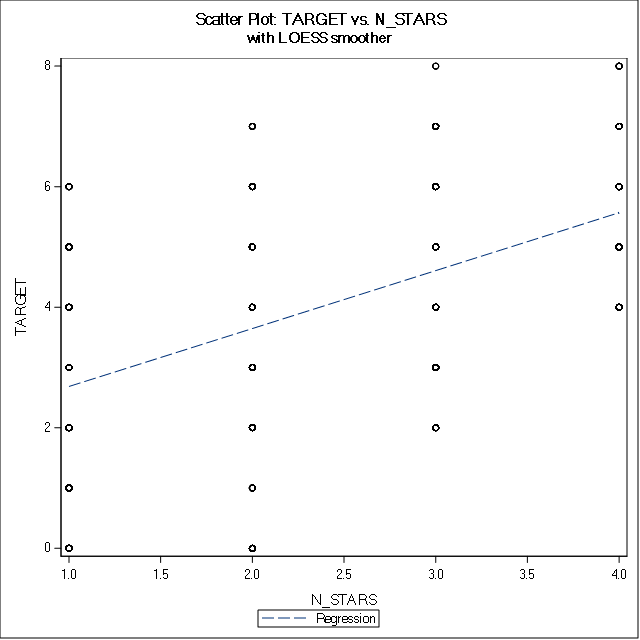
\includegraphics[height=3.95833in]{images/scatter_stars.png}

\newpage

We can immediately see the non-continuous nature of the target variable
in the scatter plots above. But perhaps more concerning is the lack of
relationship between each variable and the target. In fact, all
variables other than wine rating (N\_STARS) and appeal label
(N\_LabelAppeal) share a similar scatter plot against the target as
density (N\_Density) above.

\section{4 Data Preparation}\label{data-preparation}

The data preparation routine for this assessment follows a three step
process. This includes 1) trimming variables to account for outliers, 2)
imputing variables to account for missing values, and finally, 3)
performing a log transformation of all existing and newly created
variables. Note that during this process, new dummy variables are
created in order to reflect any identified outlier or missing
observations.

\subsection{4.1 Data Outliers}\label{data-outliers}

From the univariate analysis above, we have identified that the majority
of variables have a high amount of kurtosis and what may be considered
outlier observations. A review of the percentiles for each variable
confirms this, with a rather large gap between the min, max and the 1st
and 99th percentile for each variable. For example, levels of `total
sulfur dioxide' span -823.0mg/L to 1,057.0mg/L. Not only is it
implausible for total sulfur dioxide levels in wine to be negative, the
legal limit for sulfur dioxide in wine in the United States is 350mg/L
(N. Jackowetz 2011). It would therefore be probable that values in
excess of this are erroneous. A summary of percentiles for total sulfur
dioxide and each of the other variables can be found in the table below.

\paragraph{Table 4.1: Quantiles
Summary}\label{table-4.1-quantiles-summary}

\begin{longtable}[]{@{}llllllllllll@{}}
\toprule
Variable & Min & 0.01 & 0.05 & 0.1 & 0.25 & 0.5 & 0.75 & 0.9 & 0.95 &
0.99 & Max\tabularnewline
\midrule
\endhead
N\_FixedAcidity & -18.1 & -10.9 & -3.6 & -1.2 & 5.2 & 6.9 & 9.5 & 15.6 &
17.8 & 24.4 & 34.4\tabularnewline
N\_ResSugar & -2.8 & -1.9 & -1.0 & -0.7 & 0.1 & 0.3 & 0.6 & 1.4 & 1.6 &
2.6 & 3.7\tabularnewline
N\_CitricAcid & -3.2 & -2.2 & -1.2 & -0.8 & 0.0 & 0.3 & 0.6 & 1.4 & 1.8
& 2.7 & 3.9\tabularnewline
N\_ResSugar & -127.8 & -91.0 & -52.7 & -39.7 & -2.0 & 3.9 & 15.9 & 49.8
& 62.7 & 99.2 & 141.2\tabularnewline
N\_Chlorides & -1.2 & -0.9 & -0.5 & -0.4 & 0.0 & 0.0 & 0.2 & 0.5 & 0.6 &
1.0 & 1.4\tabularnewline
N\_FreSulfDiox & -555.0 & -388.0 & -224.0 & -171.0 & 0.0 & 30.0 & 70.0 &
230.0 & 284.0 & 469.0 & 623.0\tabularnewline
N\_TotSulfDiox & -823.0 & -531.0 & -273.0 & -185.0 & 27.0 & 123.0 &
208.0 & 422.0 & 514.0 & 767.0 & 1057.0\tabularnewline
N\_Density & 0.9 & 0.9 & 0.9 & 1.0 & 1.0 & 1.0 & 1.0 & 1.0 & 1.0 & 1.1 &
1.1\tabularnewline
N\_pH & 0.5 & 1.3 & 2.1 & 2.3 & 3.0 & 3.2 & 3.5 & 4.1 & 4.4 & 5.1 &
6.1\tabularnewline
N\_Sulphates & -3.1 & -2.1 & -1.1 & -0.7 & 0.3 & 0.5 & 0.9 & 1.8 & 2.1 &
3.2 & 4.2\tabularnewline
N\_Alcohol & -4.7 & 0.1 & 4.1 & 5.7 & 9.0 & 10.4 & 12.4 & 15.2 & 16.7 &
20.3 & 26.5\tabularnewline
N\_LabelAppeal & -2.0 & -2.0 & -1.0 & -1.0 & -1.0 & 0.0 & 1.0 & 1.0 &
1.0 & 2.0 & 2.0\tabularnewline
N\_AcidIndex & 4.0 & 6.0 & 6.0 & 7.0 & 7.0 & 8.0 & 8.0 & 9.0 & 10.0 &
13.0 & 17.0\tabularnewline
N\_STARS & 1.0 & 1.0 & 1.0 & 1.0 & 1.0 & 2.0 & 3.0 & 3.0 & 4.0 & 4.0 &
4.0\tabularnewline
\bottomrule
\end{longtable}

For this assessment, we have elected to generate trimmed copies of each
numeric variable by their 1st/99th, 5th/95th and 10th/90th percentiles.
Trimmed variables include the suffix '\_T99', '\_T95' and '\_T90'
respectively. Based on the quantile summary above, we note that the
majority of variables which are trimmed by their 1st/99th percentiles
will still retain many observations which may be classed as outliers. A
new set of dummy variables are also created in order to capture those
variables which were identified as having outlier observations according
to the percentile threshold discussed above. These dummy variables
include the suffix '\_OF'.

\subsection{4.2 Missing Data}\label{missing-data}

Following introducing copies of trimmed numeric variables, we then look
towards imputing values for missing observations. For this assessment,
we elected to impute values according to the variable's median value. By
recalculating the median value for each variable after trimming, we are
able to avoid imputing skewed values. Note that in order to simplify the
SAS logic used for this assessment, all variables will include the
suffix '\_IME', however only those variables shown to have missing
observations in the previous sections have actually received imputation.
A new set of dummy variables are also created in order to capture those
variables which were identified as having missing observations. These
variables include the suffix '\_MF'.

\subsection{4.3 Data Transformation}\label{data-transformation}

We perform a natural logarithm transformation of each of the numeric
variables. Variables which have been transformed include the suffix
'\_LN'. Such a transformation will help penalize extreme values and may
provide an improved fit within subsequent regression models. This
transformation is performed for all of the newly created variables
discussed above.

\subsection{4.4 Dummy Variables}\label{dummy-variables}

Finally, we create a number of dummy variables based on bins of wine
rating (N\_STARS) and appeal label (N\_LabelAppeal). The dummy variables
created for this assessment are detailed in the table below.

\paragraph{Table 4.2: Dummy Variable
Summary}\label{table-4.2-dummy-variable-summary}

\begin{longtable}[]{@{}ll@{}}
\toprule
Dummy & Criteria\tabularnewline
\midrule
\endhead
N\_STARS\_0 & (0.0 \textless{}= N\_STARS \textless{}
0.5);\tabularnewline
N\_STARS\_1 & (0.5 \textless{}= N\_STARS \textless{}
1.5);\tabularnewline
N\_STARS\_2 & (1.5 \textless{}= N\_STARS \textless{}
2.5);\tabularnewline
N\_STARS\_3 & (2.5 \textless{}= N\_STARS \textless{}
3.5);\tabularnewline
N\_STARS\_4 & (3.5 \textless{}= N\_STARS \textless{}=
4.0);\tabularnewline
N\_STARS\_GTE2 & (1.5 \textless{}= N\_STARS \textless{}=
4.0);\tabularnewline
N\_STARS\_GTE3 & (2.5 \textless{}= N\_STARS \textless{}=
4.0);\tabularnewline
N\_LabelAppeal\_1 & (-2.0 \textless{}= N\_LabelAppeal \textless{}
-1.5);\tabularnewline
N\_LabelAppeal\_2 & (-1.5 \textless{}= N\_LabelAppeal \textless{}
-0.5);\tabularnewline
N\_LabelAppeal\_3 & (-0.5 \textless{}= N\_LabelAppeal \textless{}
0.5);\tabularnewline
N\_LabelAppeal\_4 & (0.5 \textless{}= N\_LabelAppeal \textless{}
1.5);\tabularnewline
N\_LabelAppeal\_5 & (1.5 \textless{}= N\_LabelAppeal \textless{}=
2.0);\tabularnewline
N\_LA\_GTE3 & (-0.5 \textless{}= N\_LabelAppeal \textless{}=
2.0);\tabularnewline
N\_LA\_GTE4 & (0.5 \textless{}= N\_LabelAppeal \textless{}=
2.0);\tabularnewline
\bottomrule
\end{longtable}

Note that the newly created dummy variables include an appropriate
suffix to reflect its criteria.

\section{5 Model Development}\label{model-development}

For this section, we build five prediction models. This includes a
linear regression model and four generalized linear regression models of
the following forms; Poisson, Negative Binomial, Zero Inflated Poisson
and Zero Inflated Negative Binomial. For each model, we use a stepwise
selection technique with a SLENTRY and SLSTAY value of 0.15 in order to
determine which variables are included in each specification.

\subsection{5.1 Model 1: Linear
Regression}\label{model-1-linear-regression}

Parameter estimates for the linear regression model (Model\_LinR\_S) are
shown below.

\newpage

\paragraph{Table 5.1.1: Linear Regression Parameter
Estimates}\label{table-5.1.1-linear-regression-parameter-estimates}

\begin{longtable}[]{@{}lllllll@{}}
\toprule
Variable & DF & Est. & S.E. & t Value & \$\text{Pr} \textgreater{} &
t\tabularnewline
\midrule
\endhead
Intercept & 1 & 1.41942 & 1.79746 & 0.79 & 0.4297 & 0\tabularnewline
N\_Alcohol\_OF & 1 & 0.09899 & 0.04565 & 2.17 & 0.0301 &
1.02754\tabularnewline
N\_STARS\_1 & 1 & 1.66956 & 0.17525 & 9.53 & \textless{}.0001 &
42.05406\tabularnewline
N\_STARS\_GTE2 & 1 & 2.38672 & 0.03189 & 74.84 & \textless{}.0001 &
1.92077\tabularnewline
N\_LabelAppeal\_5 & 1 & 0.13799 & 0.06724 & 2.05 & 0.0402 &
1.25799\tabularnewline
N\_AcidIndex\_IME & 1 & -0.12299 & 0.0215 & -5.72 & \textless{}.0001 &
6.12241\tabularnewline
N\_AcidIndex\_T99\_IME & 1 & -0.58704 & 0.09362 & -6.27 &
\textless{}.0001 & 96.43776\tabularnewline
N\_Alcohol\_IME & 1 & 0.00733 & 0.00364 & 2.02 & 0.0439 &
1.31901\tabularnewline
N\_Alcohol\_T90\_IME & 1 & 0.1616 & 0.04896 & 3.3 & 0.001 &
57.08027\tabularnewline
N\_Chlorides\_IME & 1 & -0.12143 & 0.03711 & -3.27 & 0.0011 &
1.00284\tabularnewline
N\_Density\_T90\_IME & 1 & -2.22961 & 0.92926 & -2.4 & 0.0164 &
1.00357\tabularnewline
N\_FreSulfDiox\_T99\_IME & 1 & 0.00030222 & 0.0000904 & 3.34 & 0.0008 &
1.00525\tabularnewline
N\_LabelAppeal\_IME & 1 & 0.45554 & 0.01507 & 30.22 & \textless{}.0001 &
1.36263\tabularnewline
N\_STARS\_IME & 1 & 1.14507 & 0.32996 & 3.47 & 0.0005 &
494.36929\tabularnewline
N\_Sulphates\_IME & 1 & -0.03011 & 0.01299 & -2.32 & 0.0205 &
1.00297\tabularnewline
N\_TotSulfDiox\_IME & 1 & 0.00021852 & 0.00005114 & 4.27 &
\textless{}.0001 & 1.00597\tabularnewline
N\_VolAcid\_IME & 1 & -0.09513 & 0.01473 & -6.46 & \textless{}.0001 &
1.00719\tabularnewline
N\_pH\_T90\_IME & 1 & -0.13897 & 0.03582 & -3.88 & 0.0001 &
1.00728\tabularnewline
N\_AcidIndex\_T99\_IME\_LN & 1 & 4.60162 & 0.849 & 5.42 &
\textless{}.0001 & 92.23336\tabularnewline
N\_Alcohol\_T90\_IME\_LN & 1 & -1.51042 & 0.54083 & -2.79 & 0.0052 &
56.7597\tabularnewline
N\_CitricAcid\_T90\_IME\_LN & 1 & 0.11136 & 0.03953 & 2.82 & 0.0049 &
1.00515\tabularnewline
N\_STARS\_IME\_LN & 1 & -2.04254 & 1.2314 & -1.66 & 0.0972 &
749.03152\tabularnewline
\bottomrule
\end{longtable}

For Model\_LinR\_S, the majority of coefficient estimates have
significant p-values at the 95\% level, allowing us to reject the null
hypothesis and conclude that each have non-zero coefficients. The only
exception is the coefficient estimate for N\_STARS\_IME\_LN. We also
note that the VIF values for many coefficient estimates suggest that
multicollinearity may be an issue.

Goodness-of-fit information for Model\_LinR\_S is shown below.

\paragraph{Table 5.1.2: Linear Regression Analysis of
Variance}\label{table-5.1.2-linear-regression-analysis-of-variance}

\begin{longtable}[]{@{}llllll@{}}
\toprule
Source & DF & Sum of Squares & Mean Square & F Value & Pr \textgreater{}
F\tabularnewline
\midrule
\endhead
Model & 21 & 25846 & 1230.75735 & 726.75 &
\textless{}.0001\tabularnewline
Error & 12773 & 21631 & 1.69352 & &\tabularnewline
Corrected Total & 12794 & 47477 & & &\tabularnewline
\bottomrule
\end{longtable}

The model has reported a large F-value suggesting that the observations
and regression differ from the grand mean. Likewise, the F-value has a
highly significant p-value under the null hypothesis that there is no
linear relationship between the predictor and response variable.

Model performance statistics for Model\_LinR\_S are shown below.

\paragraph{Table 5.1.3: Linear Regression Performance
Metrics}\label{table-5.1.3-linear-regression-performance-metrics}

\begin{longtable}[]{@{}llll@{}}
\toprule
Measure & Statistic & Measure & Statistic\tabularnewline
\midrule
\endhead
MSE & 1.6906 & R-Square & 0.5444\tabularnewline
MAE & 1.01846 & Adj R-Sq & 0.5436\tabularnewline
Root MSE & 1.30135 & C(p) & 22\tabularnewline
Dependent Mean & 3.02907 & AIC & 6762.4748\tabularnewline
Coeff Var & 42.96203 & BIC & 6764.5506\tabularnewline
\bottomrule
\end{longtable}

The R-square value above suggests that Model\_LinR\_S explains
approximately 54\% of the variability in the target using each of the
included predictor variables. The adjusted R-squared value indicates a
similar level of explanatory power.

\subsection{5.2 Model 2: GLM: Poisson}\label{model-2-glm-poisson}

Parameter estimates for the Poisson based generalized linear model
(Model\_Poi\_S) are shown below.

\paragraph{Table 5.2.1: GLM: Poisson Parameter
Estimates}\label{table-5.2.1-glm-poisson-parameter-estimates}

\begin{longtable}[]{@{}lllllll@{}}
\toprule
Parameter & Step & DF & Est. & S.E. & Wald Chi-Square & Pr
\textgreater{} ChiSq\tabularnewline
\midrule
\endhead
Intercept & & 1 & -0.2487 & 0.4518 & 0.3 & 0.582\tabularnewline
N\_STARS\_GTE2 & & 1 & 1.0737 & 0.0183 & 3454.82 &
\textless{}.0001\tabularnewline
N\_AcidIndex\_IME & 4 & 1 & 1.2052 & 0.5481 & 4.83 &
0.0279\tabularnewline
N\_AcidIndex\_IME & 5 & 1 & 1.0712 & 0.4517 & 5.62 &
0.0177\tabularnewline
N\_AcidIndex\_IME & 6 & 1 & 1.1071 & 0.4478 & 6.11 &
0.0134\tabularnewline
N\_AcidIndex\_IME & 7 & 1 & 1.0711 & 0.4476 & 5.73 &
0.0167\tabularnewline
N\_AcidIndex\_IME & 8 & 1 & 1.0392 & 0.4476 & 5.39 &
0.0202\tabularnewline
N\_AcidIndex\_IME & 9 & 1 & 0.9271 & 0.4478 & 4.29 &
0.0384\tabularnewline
N\_AcidIndex\_IME & 10 & 1 & 0.7725 & 0.4485 & 2.97 &
0.085\tabularnewline
N\_AcidIndex\_IME & 11 & 1 & 0.4052 & 0.451 & 0.81 &
0.369\tabularnewline
N\_AcidIndex\_IME & 12 & 1 & 0.3936 & 0.4551 & 0.75 &
0.3871\tabularnewline
N\_AcidIndex\_IME & 13 & 1 & 0.5515 & 0.4572 & 1.45 &
0.2278\tabularnewline
N\_AcidIndex\_IME & 14 & 1 & 0.4552 & 0.4663 & 0.95 &
0.3289\tabularnewline
N\_AcidIndex\_IME & 15 & 1 & 0.8889 & 0.5126 & 3.01 &
0.0829\tabularnewline
N\_AcidIndex\_IME & 16 & 1 & 0.2454 & 0.6327 & 0.15 &
0.6981\tabularnewline
N\_Alcohol\_T90\_IME & & 1 & 0.0108 & 0.0029 & 14.29 &
0.0002\tabularnewline
N\_Chlorides\_IME & & 1 & -0.0383 & 0.0165 & 5.4 & 0.0201\tabularnewline
N\_LabelAppeal\_IME & -2 & 1 & -0.6994 & 0.0424 & 271.49 &
\textless{}.0001\tabularnewline
N\_LabelAppeal\_IME & -1 & 1 & -0.4574 & 0.025 & 334.89 &
\textless{}.0001\tabularnewline
N\_LabelAppeal\_IME & 0 & 1 & -0.2679 & 0.0229 & 137.24 &
\textless{}.0001\tabularnewline
N\_LabelAppeal\_IME & 1 & 1 & -0.1348 & 0.0232 & 33.83 &
\textless{}.0001\tabularnewline
N\_STARS\_IME & 1 & 1 & 0.5163 & 0.028 & 339.6 &
\textless{}.0001\tabularnewline
N\_STARS\_IME & 2 & 1 & -0.2394 & 0.0199 & 144.57 &
\textless{}.0001\tabularnewline
N\_STARS\_IME & 3 & 1 & -0.1221 & 0.0202 & 36.48 &
\textless{}.0001\tabularnewline
N\_TotSulfDiox\_IME & & 1 & 0.0001 & 0 & 10.1 & 0.0015\tabularnewline
N\_VolAcid\_IME & & 1 & -0.0291 & 0.0065 & 19.86 &
\textless{}.0001\tabularnewline
N\_pH\_T90\_IME & & 1 & -0.043 & 0.0159 & 7.3 & 0.0069\tabularnewline
N\_CitricAcid\_T90\_IME & & 1 & 0.0261 & 0.0127 & 4.22 &
0.0399\tabularnewline
N\_FreSulfDiox\_IME\_LN & & 1 & 0.0034 & 0.0013 & 6.25 &
0.0124\tabularnewline
\bottomrule
\end{longtable}

An assessment of coefficients can be achieved by taking the
\(100 \cdot (exp(\beta)-1)\) of its estimate. For example, the
coefficient estimate for N\_Alcohol\_T90\_IME suggests that a one unit
increase in alcohol translates to a 1.1\% increase in the number of wine
cases purchased. Likewise, the coefficient estimates with a step value
indicates a percentage change in the target based on that value of the
predictor. For example, the coefficient estimate for N\_LabelAppeal\_IME
with a step of -2 suggests a 50\% decrease in the amount of cases
purchased when appeal is equal to -2.

With this in mind, we are critical of a number of coefficient estimates
for the above model. For instance, we would not expect such a large
magnitude of change in the number of cases purchased from a one unit
increase in many of the included predictors. We do note that the
polarity of coefficient for the appeal variables seems appropriate.
However, it is more difficult to assess the polarity of coefficient
estimate for the chemical properties, since we are effectively assessing
perceived quality. For example, our research suggests that taste is a
balance of acidity, tannins, sugar and alcohol, with relative changes in
these quantities influencing the sweetness, sourness and bitterness
(Robinson 2006). In contrast, estimates relating to N\_VolAcid\_IME were
intuitive. The model output indicated that as the volatile acidity of
wine increases, the volume of wine purchased tends to decrease which
would be due to the increasingly unpalatable levels of acetic acid in
the wine (Neeley 2015).

The results, along with model performance criteria are shown below.

\paragraph{Table 5.2.3: GLM: Poisson Performance
Metrics}\label{table-5.2.3-glm-poisson-performance-metrics}

\begin{longtable}[]{@{}llll@{}}
\toprule
Criterion & DF & Value & Value/DF\tabularnewline
\midrule
\endhead
Deviance & 13000 & 13522.5677 & 1.0593\tabularnewline
Scaled Deviance & 13000 & 13522.5677 & 1.0593\tabularnewline
Pearson Chi-Square & 13000 & 11177.4783 & 0.8756\tabularnewline
Scaled Pearson X2 & 13000 & 11177.4783 & 0.8756\tabularnewline
Log Likelihood & & 8864.8766 &\tabularnewline
Full Log Likelihood & & -22732.2947 &\tabularnewline
AIC (smaller is better) & & 45522.5894 &\tabularnewline
AICC (smaller is better) & & 45522.7257 &\tabularnewline
BIC (smaller is better) & & 45738.8369 &\tabularnewline
\bottomrule
\end{longtable}

We note the AIC and BIC values above, as these will be used as a
comparison against other specifications.

\subsection{5.3 Model 3: GLM: Negative
Binomial}\label{model-3-glm-negative-binomial}

Parameter estimates for the Negative Binomial based generalized linear
model (Model\_NB\_S) are shown below.

\paragraph{Table 5.3.1: GLM: Negative Binomial Parameter
Estimates}\label{table-5.3.1-glm-negative-binomial-parameter-estimates}

\begin{longtable}[]{@{}lllllll@{}}
\toprule
Parameter & Step & DF & Est. & S.E. & Wald Chi-Square & Pr
\textgreater{} ChiSq\tabularnewline
\midrule
\endhead
Intercept & & 1 & -0.2487 & 0.4518 & 0.3 & 0.582\tabularnewline
N\_STARS\_GTE2 & & 1 & 1.0737 & 0.0183 & 3454.82 &
\textless{}.0001\tabularnewline
N\_AcidIndex\_IME & 4 & 1 & 1.2052 & 0.5481 & 4.83 &
0.0279\tabularnewline
N\_AcidIndex\_IME & 5 & 1 & 1.0712 & 0.4517 & 5.62 &
0.0177\tabularnewline
N\_AcidIndex\_IME & 6 & 1 & 1.1071 & 0.4478 & 6.11 &
0.0134\tabularnewline
N\_AcidIndex\_IME & 7 & 1 & 1.0711 & 0.4476 & 5.73 &
0.0167\tabularnewline
N\_AcidIndex\_IME & 8 & 1 & 1.0392 & 0.4476 & 5.39 &
0.0202\tabularnewline
N\_AcidIndex\_IME & 9 & 1 & 0.9271 & 0.4478 & 4.29 &
0.0384\tabularnewline
N\_AcidIndex\_IME & 10 & 1 & 0.7725 & 0.4485 & 2.97 &
0.085\tabularnewline
N\_AcidIndex\_IME & 11 & 1 & 0.4052 & 0.451 & 0.81 &
0.369\tabularnewline
N\_AcidIndex\_IME & 12 & 1 & 0.3936 & 0.4551 & 0.75 &
0.3871\tabularnewline
N\_AcidIndex\_IME & 13 & 1 & 0.5515 & 0.4572 & 1.45 &
0.2278\tabularnewline
N\_AcidIndex\_IME & 14 & 1 & 0.4552 & 0.4663 & 0.95 &
0.3289\tabularnewline
N\_AcidIndex\_IME & 15 & 1 & 0.8889 & 0.5126 & 3.01 &
0.0829\tabularnewline
N\_AcidIndex\_IME & 16 & 1 & 0.2454 & 0.6327 & 0.15 &
0.6981\tabularnewline
N\_Alcohol\_T90\_IME & & 1 & 0.0108 & 0.0029 & 14.29 &
0.0002\tabularnewline
N\_Chlorides\_IME & & 1 & -0.0383 & 0.0165 & 5.4 & 0.0201\tabularnewline
N\_LabelAppeal\_IME & -2 & 1 & -0.6994 & 0.0424 & 271.49 &
\textless{}.0001\tabularnewline
N\_LabelAppeal\_IME & -1 & 1 & -0.4574 & 0.025 & 334.89 &
\textless{}.0001\tabularnewline
N\_LabelAppeal\_IME & 0 & 1 & -0.2679 & 0.0229 & 137.24 &
\textless{}.0001\tabularnewline
N\_LabelAppeal\_IME & 1 & 1 & -0.1348 & 0.0232 & 33.83 &
\textless{}.0001\tabularnewline
N\_STARS\_IME & 1 & 1 & 0.5163 & 0.028 & 339.6 &
\textless{}.0001\tabularnewline
N\_STARS\_IME & 2 & 1 & -0.2394 & 0.0199 & 144.57 &
\textless{}.0001\tabularnewline
N\_STARS\_IME & 3 & 1 & -0.1221 & 0.0202 & 36.48 &
\textless{}.0001\tabularnewline
N\_TotSulfDiox\_IME & & 1 & 0.0001 & 0 & 10.1 & 0.0015\tabularnewline
N\_VolAcid\_IME & & 1 & -0.0291 & 0.0065 & 19.86 &
\textless{}.0001\tabularnewline
N\_pH\_T90\_IME & & 1 & -0.043 & 0.0159 & 7.3 & 0.0069\tabularnewline
N\_CitricAcid\_T90\_IME & & 1 & 0.0261 & 0.0127 & 4.22 &
0.0399\tabularnewline
N\_FreSulfDiox\_IME\_LN & & 1 & 0.0034 & 0.0013 & 6.25 &
0.0124\tabularnewline
\bottomrule
\end{longtable}

We see that the automated variable selection technique has mirrored the
same specification as Model\_Poi\_S. This is perhaps not surprising due
to the target variance being close to equal its mean.

Model performance statistics for Model\_NB\_S are shown below.

\paragraph{Table 5.3.2: GLM: Negative Binomial Performance
Metrics}\label{table-5.3.2-glm-negative-binomial-performance-metrics}

\begin{longtable}[]{@{}llll@{}}
\toprule
Criterion & DF & Value & Value/DF\tabularnewline
\midrule
\endhead
Deviance & 13000 & 13522.5677 & 1.0593\tabularnewline
Scaled Deviance & 13000 & 13522.5677 & 1.0593\tabularnewline
Pearson Chi-Square & 13000 & 11177.4694 & 0.8756\tabularnewline
Scaled Pearson X2 & 13000 & 11177.4694 & 0.8756\tabularnewline
Log Likelihood & & 8864.8766 &\tabularnewline
Full Log Likelihood & & -22732.2947 &\tabularnewline
AIC (smaller is better) & & 45524.5894 &\tabularnewline
AICC (smaller is better) & & 45524.7351 &\tabularnewline
BIC (smaller is better) & & 45748.2937 &\tabularnewline
\bottomrule
\end{longtable}

We see that the AIC and BIC for Model\_NB\_S is slightly higher (worse)
than that of Model\_Poi\_S. However, there is no difference between the
ratio of deviance to degree of freedom. We may have expected a Negative
Binomial based model to perform better than a Poisson based model, as it
allows for some overdispersion, however in this case, it seems that
overdispersion is not an issue.

\subsection{5.4 Model 4: GLM: Zero Inflated
Poisson}\label{model-4-glm-zero-inflated-poisson}

Parameter estimates for the Zero Inflated Poisson generalized linear
model (Model\_ZPoi\_S) are shown below.

\paragraph{Table 5.4.1: GLM: Poisson Parameter
Estimates}\label{table-5.4.1-glm-poisson-parameter-estimates}

\begin{longtable}[]{@{}lllllll@{}}
\toprule
Parameter & Step & DF & Est. & S.E. & Wald Chi-Square & Pr
\textgreater{} ChiSq\tabularnewline
\midrule
\endhead
Intercept & & 1 & 1.4688 & 0.0677 & 470.47 &
\textless{}.0001\tabularnewline
N\_STARS\_GTE2 & & 1 & 0.4752 & 0.0285 & 277.32 &
\textless{}.0001\tabularnewline
N\_AcidIndex\_T95\_IME & & 1 & -0.0249 & 0.006 & 17.46 &
\textless{}.0001\tabularnewline
N\_Alcohol\_IME & & 1 & 0.0041 & 0.0017 & 6.21 & 0.0127\tabularnewline
N\_Alcohol\_T90\_IME & & 1 & 0.0095 & 0.0034 & 8.04 &
0.0046\tabularnewline
N\_LabelAppeal\_IME & -2 & 1 & -1.0236 & 0.0458 & 499.52 &
\textless{}.0001\tabularnewline
N\_LabelAppeal\_IME & -1 & 1 & -0.6331 & 0.026 & 591.12 &
\textless{}.0001\tabularnewline
N\_LabelAppeal\_IME & 0 & 1 & -0.3518 & 0.0233 & 227.54 &
\textless{}.0001\tabularnewline
N\_LabelAppeal\_IME & 1 & 1 & -0.1637 & 0.0235 & 48.45 &
\textless{}.0001\tabularnewline
N\_STARS\_IME & 1 & 1 & 0.1579 & 0.0351 & 20.23 &
\textless{}.0001\tabularnewline
N\_STARS\_IME & 2 & 1 & -0.1822 & 0.0199 & 83.38 &
\textless{}.0001\tabularnewline
N\_STARS\_IME & 3 & 1 & -0.099 & 0.0202 & 24.03 &
\textless{}.0001\tabularnewline
N\_VolAcid\_IME & & 1 & -0.018 & 0.0068 & 7.02 & 0.008\tabularnewline
\bottomrule
\end{longtable}

\paragraph{Table 5.4.2: GLM: Zero Inflated Poisson Parameter
Estimates}\label{table-5.4.2-glm-zero-inflated-poisson-parameter-estimates}

\begin{longtable}[]{@{}lllllll@{}}
\toprule
Parameter & & DF & Est. & S.E. & Wald Chi-Square & Pr \textgreater{}
ChiSq\tabularnewline
\midrule
\endhead
Intercept & & 1 & -4.394 & 756.2719 & 0 & 0.9954\tabularnewline
N\_STARS\_IME & 1 & 1 & 18.2319 & 674.7371 & 0 & 0.9784\tabularnewline
N\_STARS\_IME & 2 & 1 & 18.5193 & 674.7371 & 0 & 0.9781\tabularnewline
N\_STARS\_IME & 3 & 1 & -7.4969 & 796.0038 & 0 & 0.9925\tabularnewline
N\_LabelAppeal\_IME & -2 & 1 & -2.8423 & 0.5858 & 23.54 &
\textless{}.0001\tabularnewline
N\_LabelAppeal\_IME & -1 & 1 & -1.4548 & 0.1697 & 73.47 &
\textless{}.0001\tabularnewline
N\_LabelAppeal\_IME & 0 & 1 & -0.8331 & 0.1493 & 31.16 &
\textless{}.0001\tabularnewline
N\_LabelAppeal\_IME & 1 & 1 & -0.4174 & 0.1518 & 7.56 &
0.006\tabularnewline
N\_AcidIndex\_IME & 4 & 1 & -13.7932 & 341.5851 & 0 &
0.9678\tabularnewline
N\_AcidIndex\_IME & 5 & 1 & -15.3206 & 341.5814 & 0 &
0.9642\tabularnewline
N\_AcidIndex\_IME & 6 & 1 & -15.0953 & 341.581 & 0 &
0.9648\tabularnewline
N\_AcidIndex\_IME & 7 & 1 & -15.032 & 341.581 & 0 &
0.9649\tabularnewline
N\_AcidIndex\_IME & 8 & 1 & -14.703 & 341.581 & 0 &
0.9657\tabularnewline
N\_AcidIndex\_IME & 9 & 1 & -14.0103 & 341.581 & 0 &
0.9673\tabularnewline
N\_AcidIndex\_IME & 10 & 1 & -13.331 & 341.581 & 0 &
0.9689\tabularnewline
N\_AcidIndex\_IME & 11 & 1 & -12.3995 & 341.581 & 0 &
0.971\tabularnewline
N\_AcidIndex\_IME & 12 & 1 & -12.072 & 341.5811 & 0 &
0.9718\tabularnewline
N\_AcidIndex\_IME & 13 & 1 & -12.4809 & 341.5811 & 0 &
0.9709\tabularnewline
N\_AcidIndex\_IME & 14 & 1 & -12.1375 & 341.5812 & 0 &
0.9717\tabularnewline
N\_AcidIndex\_IME & 15 & 1 & -13.3732 & 341.582 & 0 &
0.9688\tabularnewline
N\_AcidIndex\_IME & 16 & 1 & 0.3679 & 434.0462 & 0 &
0.9993\tabularnewline
\bottomrule
\end{longtable}

We again note similarity in the final predictors included for
Model\_ZPoi\_S and the previously discussed models. However, the zero
inflated parameter estimates suggest that the above model has aided in
treating the high amount of zero observations within the label appeal
variable. The key difference between this and earlier models is the
production of two tables - the Poisson Count Model and Logit Model for
Predicting Excess Zeros. (Digital Research and Education 2016) notes
that this approach assumes that the excess zeros in the model are
produced by a separate process and therefore need to be modelled
independently.

Similar to other models tested above, the estimates for N\_STARS\_IME
are not intuitive. The data dictionary defines wines with higher STARS
ratings (e.g.~3-4 stars) as being of a higher quality than wines with
lower STARS ratings (e.g.~1-2 stars). However, the parameter estimates
show that higher STARS ratings do not necessarily correspond with more
wine purchases.

Model performance statistics for Model\_ZPoi\_S are shown below.

\paragraph{Table 5.4.3: GLM: Zero Inflated Poisson Performance
Metrics}\label{table-5.4.3-glm-zero-inflated-poisson-performance-metrics}

\begin{longtable}[]{@{}llll@{}}
\toprule
Criterion & DF & Value & Value/DF\tabularnewline
\midrule
\endhead
Deviance & & 43577.0023 &\tabularnewline
Scaled Deviance & & 43577.0023 &\tabularnewline
Pearson Chi-Square & 13000 & 6704.5151 & 0.5254\tabularnewline
Scaled Pearson X2 & 13000 & 6704.5151 & 0.5254\tabularnewline
Log Likelihood & & 9808.6701 &\tabularnewline
Full Log Likelihood & & -21788.5011 &\tabularnewline
AIC (smaller is better) & & 43645.0023 &\tabularnewline
AICC (smaller is better) & & 43645.1888 &\tabularnewline
BIC (smaller is better) & & 43898.5338 &\tabularnewline
\bottomrule
\end{longtable}

We see an improvement in both the AIC and BIC for Model\_ZPoi\_S is
lower (better) than that of Model\_Poi\_S.

\subsection{5.5 Model 5: GLM: Zero Inflated Negative
Binomial}\label{model-5-glm-zero-inflated-negative-binomial}

Parameter estimates for the Zero Inflated Poisson generalized linear
model (Model\_ZNB\_S) are shown below.

\paragraph{Table 5.5.1: GLM: Negative Binomial Parameter
Estimates}\label{table-5.5.1-glm-negative-binomial-parameter-estimates}

\begin{longtable}[]{@{}lllllll@{}}
\toprule
Parameter & Step & DF & Est. & S.E. & Wald Chi-Square & Pr
\textgreater{} ChiSq\tabularnewline
\midrule
\endhead
Intercept & & 1 & 1.4629 & 0.0681 & 461.64 &
\textless{}.0001\tabularnewline
N\_STARS\_GTE2 & & 1 & 0.4813 & 0.0289 & 278.01 &
\textless{}.0001\tabularnewline
N\_AcidIndex\_T95\_IME & & 1 & -0.0249 & 0.006 & 17.25 &
\textless{}.0001\tabularnewline
N\_Alcohol\_IME & & 1 & 0.0042 & 0.0017 & 6.25 & 0.0124\tabularnewline
N\_Alcohol\_T90\_IME & & 1 & 0.0094 & 0.0034 & 7.79 &
0.0053\tabularnewline
N\_LabelAppeal\_IME & -2 & 1 & -1.0086 & 0.0456 & 490.13 &
\textless{}.0001\tabularnewline
N\_LabelAppeal\_IME & -1 & 1 & -0.6308 & 0.0262 & 579.38 &
\textless{}.0001\tabularnewline
N\_LabelAppeal\_IME & 0 & 1 & -0.3507 & 0.0235 & 222.94 &
\textless{}.0001\tabularnewline
N\_LabelAppeal\_IME & 1 & 1 & -0.1633 & 0.0237 & 47.57 &
\textless{}.0001\tabularnewline
N\_STARS\_IME & 1 & 1 & 0.1625 & 0.0354 & 21.08 &
\textless{}.0001\tabularnewline
N\_STARS\_IME & 2 & 1 & -0.1828 & 0.02 & 83.12 &
\textless{}.0001\tabularnewline
N\_STARS\_IME & 3 & 1 & -0.0994 & 0.0203 & 23.94 &
\textless{}.0001\tabularnewline
N\_VolAcid\_IME & & 1 & -0.0185 & 0.0068 & 7.4 & 0.0065\tabularnewline
\bottomrule
\end{longtable}

The Negative Binomial Parameter Estimates technique has produced similar
results to Model\_ZPoi\_S and the previously discussed models.

\paragraph{Table 5.5.2: GLM: Zero Inflated Negative Binomial Parameter
Estimates}\label{table-5.5.2-glm-zero-inflated-negative-binomial-parameter-estimates}

\begin{longtable}[]{@{}lllllll@{}}
\toprule
Parameter & & DF & Est. & S.E. & Wald Chi-Square & Pr \textgreater{}
ChiSq\tabularnewline
\midrule
\endhead
Intercept & & 1 & -6.8329 & 1.354 & 25.47 &
\textless{}.0001\tabularnewline
N\_STARS\_IME & 1 & 1 & 3.2252 & 0.3943 & 66.9 &
\textless{}.0001\tabularnewline
N\_STARS\_IME & 2 & 1 & 3.521 & 0.3912 & 81.02 &
\textless{}.0001\tabularnewline
N\_STARS\_IME & 3 & 1 & -0.8452 & 0.5111 & 2.73 & 0.0982\tabularnewline
N\_LabelAppeal\_IME & -2 & 1 & -2.3416 & 0.4016 & 34 &
\textless{}.0001\tabularnewline
N\_LabelAppeal\_IME & -1 & 1 & -1.4016 & 0.1678 & 69.76 &
\textless{}.0001\tabularnewline
N\_LabelAppeal\_IME & 0 & 1 & -0.7878 & 0.1476 & 28.49 &
\textless{}.0001\tabularnewline
N\_LabelAppeal\_IME & 1 & 1 & -0.3817 & 0.1499 & 6.49 &
0.0109\tabularnewline
N\_AcidIndex\_IME & 4 & 1 & 3.8158 & 2.0135 & 3.59 &
0.0581\tabularnewline
N\_AcidIndex\_IME & 5 & 1 & 2.2842 & 1.3622 & 2.81 &
0.0936\tabularnewline
N\_AcidIndex\_IME & 6 & 1 & 2.3033 & 1.2944 & 3.17 &
0.0752\tabularnewline
N\_AcidIndex\_IME & 7 & 1 & 2.3539 & 1.2895 & 3.33 &
0.0679\tabularnewline
N\_AcidIndex\_IME & 8 & 1 & 2.6837 & 1.2897 & 4.33 &
0.0375\tabularnewline
N\_AcidIndex\_IME & 9 & 1 & 3.3782 & 1.2912 & 6.85 &
0.0089\tabularnewline
N\_AcidIndex\_IME & 10 & 1 & 4.0638 & 1.2939 & 9.86 &
0.0017\tabularnewline
N\_AcidIndex\_IME & 11 & 1 & 4.989 & 1.299 & 14.75 &
0.0001\tabularnewline
N\_AcidIndex\_IME & 12 & 1 & 5.2714 & 1.3105 & 16.18 &
\textless{}.0001\tabularnewline
N\_AcidIndex\_IME & 13 & 1 & 4.9162 & 1.3232 & 13.8 &
0.0002\tabularnewline
N\_AcidIndex\_IME & 14 & 1 & 5.2288 & 1.3404 & 15.22 &
\textless{}.0001\tabularnewline
N\_AcidIndex\_IME & 15 & 0 & 4.2238 & 0 & . & .\tabularnewline
N\_AcidIndex\_IME & 16 & 1 & 4.3348 & 1.7154 & 6.39 &
0.0115\tabularnewline
\bottomrule
\end{longtable}

Model performance statistics for Model\_ZNB\_S are shown below.

\paragraph{Table 5.5.3: GLM: Zero Inflated Negative Binomial Performance
Metrics}\label{table-5.5.3-glm-zero-inflated-negative-binomial-performance-metrics}

\begin{longtable}[]{@{}llll@{}}
\toprule
Criterion & DF & Value & Value/DF\tabularnewline
\midrule
\endhead
Deviance & & 43695.6413 &\tabularnewline
Scaled Deviance & & 43695.6413 &\tabularnewline
Pearson Chi-Square & 13000 & 6695.4366 & 0.5247\tabularnewline
Scaled Pearson X2 & 13000 & 6695.4366 & 0.5247\tabularnewline
Log Likelihood & & -21847.8206 &\tabularnewline
Full Log Likelihood & & -21847.8206 &\tabularnewline
AIC (smaller is better) & & 43765.6413 &\tabularnewline
AICC (smaller is better) & & 43765.8388 &\tabularnewline
BIC (smaller is better) & & 44026.6296 &\tabularnewline
\bottomrule
\end{longtable}

\section{6 Model Selection}\label{model-selection}

In order to select the optimum model, we have collated and assessed the
AIC, AICC and BIC of each. A summary of performance metrics over each
model is shown below.

\paragraph{Table 6.1: Model Performance Metric
Summary}\label{table-6.1-model-performance-metric-summary}

\begin{longtable}[]{@{}llll@{}}
\toprule
Model & AIC & AICC & BIC\tabularnewline
\midrule
\endhead
Model\_Poi\_S & 45522.5894 & 45522.7257 & 45738.8369\tabularnewline
Model\_NB\_S & 45524.5894 & 45524.7351 & 45748.2937\tabularnewline
Model\_ZPoi\_S & 43645.0023 & 43645.1888 & 43898.5338\tabularnewline
Model\_ZNB\_S & 43765.6413 & 43765.8388 & 44026.6296\tabularnewline
\bottomrule
\end{longtable}

Based on the results above, this assessment concludes that
Model\_ZPoi\_S is the superior model. Its performance metrics were among
the most favorable, and maintained a ratio of deviance to degree of
freedom close to one.

\section{7 Model Deployment Code}\label{model-deployment-code}

Please see Appendix A for the final deployment code.

\section{8 Conclusion}\label{conclusion}

Five predictive models were built, each specified using automated
variable selection techniques, and we predicted the number of wine
orders based on a withheld test set of data using a SAS routine. To
assess the performance of each model we compared the AIC, AICC and BIC
values. The Zero Inflated Poisson model produced the most favorable
performance metrics, with the lowest AIC, AICC and BIC metrics of all
the models tested. In addition, the Zero Inflated Poisson model
maintained a ratio of deviance to degree of freedom close to one.

\newpage

\section{Appendix A: Final Deployment
Code}\label{appendix-a-final-deployment-code}

\begin{Shaded}
\begin{Highlighting}[]

\CommentTok{* Set variables / global macros;}

\NormalTok{%LET key }\KeywordTok{=} \KeywordTok{INDEX}\NormalTok{;}
\NormalTok{%LET response }\KeywordTok{=} \DataTypeTok{TARGET}\NormalTok{;}
\NormalTok{%LET varname }\KeywordTok{=} \NormalTok{name;}

\NormalTok{%LET data }\KeywordTok{=} \NormalTok{wine;}
\NormalTok{%LET contents }\KeywordTok{=} \KeywordTok{&}\NormalTok{data._contents;}



\CommentTok{* Load the dataset;}

\NormalTok{libname mydata }\StringTok{'/sscc/home/d/dgb2583/411/'} \FunctionTok{access} \KeywordTok{=} \NormalTok{readonly;}

\DataTypeTok{DATA} \KeywordTok{&}\NormalTok{data.;}
    \KeywordTok{*}\NormalTok{SET mydata.wine;}
    \NormalTok{SET mydata.wine_test;}
\NormalTok{RUN; QUIT;}

\NormalTok{PROC CONTENTS DATA }\KeywordTok{=} \KeywordTok{&}\NormalTok{data. OUT }\KeywordTok{=} \KeywordTok{&}\NormalTok{contents.;}
\NormalTok{RUN; QUIT;}

\CommentTok{*PROC PRINT DATA = &contents. (OBS=20);}
\CommentTok{*RUN; QUIT;}

\NormalTok{PROC MEANS DATA }\KeywordTok{=} \KeywordTok{&}\NormalTok{data. }\KeywordTok{MIN} \NormalTok{P5 P50 P90 P95 P99 }\KeywordTok{MAX} \NormalTok{MEAN STDDEV NMISS N;}
\NormalTok{RUN; QUIT;}



\CommentTok{* Data rename;}

\NormalTok{%MACRO rename_num(varname);}
\DataTypeTok{    DATA} \KeywordTok{&}\NormalTok{data_def.;}
        \NormalTok{SET }\KeywordTok{&}\NormalTok{data_def. (RENAME }\KeywordTok{=} \NormalTok{(}\KeywordTok{&}\NormalTok{varname. }\KeywordTok{=} \NormalTok{N_}\KeywordTok{&}\NormalTok{varname.));}
    \NormalTok{RUN; QUIT;}
\NormalTok{%MEND;}

\NormalTok{TITLE1 }\StringTok{''}\NormalTok{;}
\NormalTok{TITLE2 }\StringTok{''}\NormalTok{;}

\DataTypeTok{DATA} \KeywordTok{&}\NormalTok{data._name;}
    \NormalTok{SET }\KeywordTok{&}\NormalTok{data.}
        \NormalTok{(RENAME }\KeywordTok{=} \NormalTok{(TotalSulfurDioxide   }\KeywordTok{=} \NormalTok{TotSulfDiox}
                   \NormalTok{FreeSulfurDioxide    }\KeywordTok{=} \NormalTok{FreSulfDiox}
                   \NormalTok{ResidualSugar        }\KeywordTok{=} \NormalTok{ResSugar}
                   \NormalTok{VolatileAcidity      }\KeywordTok{=} \NormalTok{VolAcid));}
\NormalTok{RUN; QUIT;}

\NormalTok{PROC CONTENTS DATA }\KeywordTok{=} \KeywordTok{&}\NormalTok{data._name OUT }\KeywordTok{=} \KeywordTok{&}\NormalTok{contents._name;}
\NormalTok{RUN; QUIT;}

\DataTypeTok{DATA} \KeywordTok{&}\NormalTok{contents._name;}
    \NormalTok{SET }\KeywordTok{&}\NormalTok{contents._name;}
        \KeywordTok{IF} \NormalTok{name }\KeywordTok{=} \StringTok{"&key."} \KeywordTok{then} \NormalTok{DELETE;}
        \KeywordTok{IF} \NormalTok{name }\KeywordTok{=} \StringTok{"&response."} \KeywordTok{then} \NormalTok{DELETE;}
\NormalTok{RUN; QUIT;}

\NormalTok{%LET data_def }\KeywordTok{=} \KeywordTok{&}\NormalTok{data._name;}

\DataTypeTok{DATA} \NormalTok{_null_;}
    \KeywordTok{DO} \NormalTok{i }\KeywordTok{=} \DecValTok{1} \KeywordTok{to} \NormalTok{NUM;}
        \NormalTok{SET }\KeywordTok{&}\NormalTok{contents._name NOBS }\KeywordTok{=} \NormalTok{NUM;}
            \KeywordTok{WHERE} \DataTypeTok{type} \KeywordTok{=} \DecValTok{1}\NormalTok{;}
                \KeywordTok{CALL} \NormalTok{EXECUTE(}\StringTok{'%rename_num('}\KeywordTok{||}\NormalTok{name}\KeywordTok{||}\StringTok{')'}\NormalTok{);}
    \KeywordTok{END}\NormalTok{;}
\NormalTok{RUN; QUIT;}

\NormalTok{PROC MEANS DATA }\KeywordTok{=} \KeywordTok{&}\NormalTok{data._name }\KeywordTok{MIN} \NormalTok{P5 P50 P90 P95 P99 }\KeywordTok{MAX} \NormalTok{MEAN STDDEV NMISS N;}
\NormalTok{RUN; QUIT;}

\NormalTok{PROC CONTENTS DATA }\KeywordTok{=} \KeywordTok{&}\NormalTok{data._name OUT }\KeywordTok{=} \KeywordTok{&}\NormalTok{contents._name;}
\NormalTok{RUN; QUIT;}



\CommentTok{* Data preparation;}

\NormalTok{%MACRO means(varname);}
    \NormalTok{PROC means DATA }\KeywordTok{=} \KeywordTok{&}\NormalTok{data_def. noprint;}
    \NormalTok{OUTPUT OUT }\KeywordTok{=} \KeywordTok{&}\NormalTok{varname. (DROP }\KeywordTok{=} \NormalTok{_freq_ _type_)}
        \NormalTok{nmiss(}\KeywordTok{&}\NormalTok{varname.)    }\KeywordTok{=} \KeywordTok{&}\NormalTok{varname._nmiss}
        \NormalTok{n(}\KeywordTok{&}\NormalTok{varname.)        }\KeywordTok{=} \KeywordTok{&}\NormalTok{varname._n}
        \NormalTok{mean(}\KeywordTok{&}\NormalTok{varname.)     }\KeywordTok{=} \KeywordTok{&}\NormalTok{varname._mean}
        \NormalTok{median(}\KeywordTok{&}\NormalTok{varname.)   }\KeywordTok{=} \KeywordTok{&}\NormalTok{varname._median}
        \NormalTok{mode(}\KeywordTok{&}\NormalTok{varname.)     }\KeywordTok{=} \KeywordTok{&}\NormalTok{varname._mode}
        \NormalTok{std(}\KeywordTok{&}\NormalTok{varname.)      }\KeywordTok{=} \KeywordTok{&}\NormalTok{varname._std}
        \NormalTok{skew(}\KeywordTok{&}\NormalTok{varname.)     }\KeywordTok{=} \KeywordTok{&}\NormalTok{varname._skew}
        \NormalTok{P1(}\KeywordTok{&}\NormalTok{varname.)       }\KeywordTok{=} \KeywordTok{&}\NormalTok{varname._P1}
        \NormalTok{P5(}\KeywordTok{&}\NormalTok{varname.)       }\KeywordTok{=} \KeywordTok{&}\NormalTok{varname._P5}
        \NormalTok{P10(}\KeywordTok{&}\NormalTok{varname.)      }\KeywordTok{=} \KeywordTok{&}\NormalTok{varname._P10}
        \NormalTok{P25(}\KeywordTok{&}\NormalTok{varname.)      }\KeywordTok{=} \KeywordTok{&}\NormalTok{varname._P25}
        \NormalTok{P50(}\KeywordTok{&}\NormalTok{varname.)      }\KeywordTok{=} \KeywordTok{&}\NormalTok{varname._P50}
        \NormalTok{P75(}\KeywordTok{&}\NormalTok{varname.)      }\KeywordTok{=} \KeywordTok{&}\NormalTok{varname._P75}
        \NormalTok{P90(}\KeywordTok{&}\NormalTok{varname.)      }\KeywordTok{=} \KeywordTok{&}\NormalTok{varname._P90}
        \NormalTok{P95(}\KeywordTok{&}\NormalTok{varname.)      }\KeywordTok{=} \KeywordTok{&}\NormalTok{varname._P95}
        \NormalTok{P99(}\KeywordTok{&}\NormalTok{varname.)      }\KeywordTok{=} \KeywordTok{&}\NormalTok{varname._P99}
        \KeywordTok{min}\NormalTok{(}\KeywordTok{&}\NormalTok{varname.)      }\KeywordTok{=} \KeywordTok{&}\NormalTok{varname._min}
        \KeywordTok{max}\NormalTok{(}\KeywordTok{&}\NormalTok{varname.)      }\KeywordTok{=} \KeywordTok{&}\NormalTok{varname._max}
        \NormalTok{qrange(}\KeywordTok{&}\NormalTok{varname.)   }\KeywordTok{=} \KeywordTok{&}\NormalTok{varname._qrange}
        \NormalTok{;}
    \NormalTok{RUN; QUIT;}
\NormalTok{%MEND;}

\NormalTok{%MACRO }\FunctionTok{transpose}\NormalTok{(varname);}
    \NormalTok{PROC }\FunctionTok{transpose} \NormalTok{DATA }\KeywordTok{=} \KeywordTok{&}\NormalTok{varname. OUT }\KeywordTok{=} \KeywordTok{&}\NormalTok{varname._t;}
        \NormalTok{var _numeric_;}
    \NormalTok{RUN; QUIT;}
\NormalTok{%MEND;}

\NormalTok{%MACRO symputx_num(varname);}
\DataTypeTok{    DATA} \NormalTok{_null_;}
        \NormalTok{SET }\KeywordTok{&}\NormalTok{varname._t;}
            \KeywordTok{CALL} \NormalTok{symputx(_name_, strip(col1), }\StringTok{'g'}\NormalTok{);}
    \NormalTok{RUN; QUIT;}
\NormalTok{%MEND;}

\NormalTok{%MACRO outlier(varname);}
\DataTypeTok{    DATA} \KeywordTok{&}\NormalTok{data_def.;}
        \NormalTok{SET }\KeywordTok{&}\NormalTok{data_def.;}
            \KeywordTok{*IF} \NormalTok{(}\KeywordTok{&}\NormalTok{varname. }\KeywordTok{<} \KeywordTok{&&&}\NormalTok{varname._P10) OR (}\KeywordTok{&}\NormalTok{varname. }\KeywordTok{>} \KeywordTok{&&&}\NormalTok{varname._P90) }\KeywordTok{THEN}
            \KeywordTok{*}   \KeywordTok{&}\NormalTok{varname._OF }\KeywordTok{=} \FloatTok{1.0}\NormalTok{; }\KeywordTok{*ELSE} \KeywordTok{&}\NormalTok{varname._OF }\KeywordTok{=} \FloatTok{0.0}\NormalTok{;}
            
            \KeywordTok{*IF} \NormalTok{(}\KeywordTok{&}\NormalTok{varname. }\KeywordTok{<} \KeywordTok{&&&}\NormalTok{varname._P5) OR (}\KeywordTok{&}\NormalTok{varname. }\KeywordTok{>} \KeywordTok{&&&}\NormalTok{varname._P95) }\KeywordTok{THEN}
            \KeywordTok{*}   \KeywordTok{&}\NormalTok{varname._OF }\KeywordTok{=} \FloatTok{1.0}\NormalTok{; }\KeywordTok{*ELSE} \KeywordTok{&}\NormalTok{varname._OF }\KeywordTok{=} \FloatTok{0.0}\NormalTok{;}
            
            \KeywordTok{IF} \NormalTok{(}\KeywordTok{&}\NormalTok{varname. }\KeywordTok{<} \KeywordTok{&&&}\NormalTok{varname._P1) OR (}\KeywordTok{&}\NormalTok{varname. }\KeywordTok{>} \KeywordTok{&&&}\NormalTok{varname._P99) }\KeywordTok{THEN}
                \KeywordTok{&}\NormalTok{varname._OF }\KeywordTok{=} \FloatTok{1.0}\NormalTok{; }\KeywordTok{ELSE} \KeywordTok{&}\NormalTok{varname._OF }\KeywordTok{=} \FloatTok{0.0}\NormalTok{;}
    \NormalTok{RUN; QUIT;}
\NormalTok{%MEND;}

\NormalTok{%MACRO }\FunctionTok{trim}\NormalTok{(varname);}
\DataTypeTok{    DATA} \KeywordTok{&}\NormalTok{data_def.;}
        \NormalTok{SET }\KeywordTok{&}\NormalTok{data_def.;}
            \KeywordTok{&}\NormalTok{varname._T90 }\KeywordTok{=} \KeywordTok{&}\NormalTok{varname.;}
            \KeywordTok{*&}\NormalTok{varname._T90 }\KeywordTok{=} \KeywordTok{max}\NormalTok{(}\KeywordTok{min}\NormalTok{(}\KeywordTok{&}\NormalTok{varname.,}\KeywordTok{&&&}\NormalTok{varname._P90),}\KeywordTok{&&&}\NormalTok{varname._P10);}
            \KeywordTok{IF} \NormalTok{(}\KeywordTok{&}\NormalTok{varname._T90 }\KeywordTok{<} \KeywordTok{&&&}\NormalTok{varname._P10) OR (}\KeywordTok{&}\NormalTok{varname._T90 }\KeywordTok{>} \KeywordTok{&&&}\NormalTok{varname._P90) }\KeywordTok{THEN}
                \KeywordTok{&}\NormalTok{varname._T90 }\KeywordTok{=} \StringTok{'.'}\NormalTok{;}
            
            \KeywordTok{&}\NormalTok{varname._T95 }\KeywordTok{=} \KeywordTok{&}\NormalTok{varname.;}
            \KeywordTok{*&}\NormalTok{varname._T95 }\KeywordTok{=} \KeywordTok{max}\NormalTok{(}\KeywordTok{min}\NormalTok{(}\KeywordTok{&}\NormalTok{varname.,}\KeywordTok{&&&}\NormalTok{varname._P95),}\KeywordTok{&&&}\NormalTok{varname._P5);}
            \KeywordTok{IF} \NormalTok{(}\KeywordTok{&}\NormalTok{varname._T95 }\KeywordTok{<} \KeywordTok{&&&}\NormalTok{varname._P5) OR (}\KeywordTok{&}\NormalTok{varname._T95 }\KeywordTok{>} \KeywordTok{&&&}\NormalTok{varname._P95) }\KeywordTok{THEN}
                \KeywordTok{&}\NormalTok{varname._T95 }\KeywordTok{=} \StringTok{'.'}\NormalTok{;}
            
            \KeywordTok{&}\NormalTok{varname._T99 }\KeywordTok{=} \KeywordTok{&}\NormalTok{varname.;}
            \KeywordTok{*&}\NormalTok{varname._T99 }\KeywordTok{=} \KeywordTok{max}\NormalTok{(}\KeywordTok{min}\NormalTok{(}\KeywordTok{&}\NormalTok{varname.,}\KeywordTok{&&&}\NormalTok{varname._P99),}\KeywordTok{&&&}\NormalTok{varname._P1);}
            \KeywordTok{IF} \NormalTok{(}\KeywordTok{&}\NormalTok{varname._T99 }\KeywordTok{<} \KeywordTok{&&&}\NormalTok{varname._P1) OR (}\KeywordTok{&}\NormalTok{varname._T99 }\KeywordTok{>} \KeywordTok{&&&}\NormalTok{varname._P99) }\KeywordTok{THEN}
                \KeywordTok{&}\NormalTok{varname._T99 }\KeywordTok{=} \StringTok{'.'}\NormalTok{;}
    \NormalTok{RUN; QUIT;}
\NormalTok{%MEND;}

\NormalTok{%MACRO missing(varname);}
\DataTypeTok{    DATA} \KeywordTok{&}\NormalTok{data_def.;}
        \NormalTok{SET }\KeywordTok{&}\NormalTok{data_def.;}
            \KeywordTok{IF} \NormalTok{missing(}\KeywordTok{&}\NormalTok{varname.) }\KeywordTok{THEN}
                \KeywordTok{&}\NormalTok{varname._MF }\KeywordTok{=} \FloatTok{1.0}\NormalTok{; }\KeywordTok{ELSE} \KeywordTok{&}\NormalTok{varname._MF }\KeywordTok{=} \FloatTok{0.0}\NormalTok{;}
    \NormalTok{RUN; QUIT;}
\NormalTok{%MEND;}

\NormalTok{%MACRO impute(varname);}
\DataTypeTok{    DATA} \KeywordTok{&}\NormalTok{data_def.;}
        \NormalTok{SET }\KeywordTok{&}\NormalTok{data_def.;}
            \KeywordTok{*&}\NormalTok{varname._IMU }\KeywordTok{=} \KeywordTok{&}\NormalTok{varname.;}
            \KeywordTok{*IF} \NormalTok{missing(}\KeywordTok{&}\NormalTok{varname._IMU) }\KeywordTok{THEN}
            \KeywordTok{*}   \KeywordTok{&}\NormalTok{varname._IMU }\KeywordTok{=} \KeywordTok{&&&}\NormalTok{varname._mean;}
            
            \KeywordTok{*&}\NormalTok{varname._IMO }\KeywordTok{=} \KeywordTok{&}\NormalTok{varname.;}
            \KeywordTok{*IF} \NormalTok{missing(}\KeywordTok{&}\NormalTok{varname._IMO) }\KeywordTok{THEN}
            \KeywordTok{*}   \KeywordTok{&}\NormalTok{varname._IMO }\KeywordTok{=} \KeywordTok{&&&}\NormalTok{varname._mode;}
            
            \KeywordTok{&}\NormalTok{varname._IME }\KeywordTok{=} \KeywordTok{&}\NormalTok{varname.;}
            \KeywordTok{IF} \NormalTok{missing(}\KeywordTok{&}\NormalTok{varname._IME) }\KeywordTok{THEN}
                \KeywordTok{&}\NormalTok{varname._IME }\KeywordTok{=} \KeywordTok{&&&}\NormalTok{varname._median;}
    \NormalTok{RUN; QUIT;}
\NormalTok{%MEND;}

\NormalTok{%MACRO transform(varname);}
\DataTypeTok{    DATA} \KeywordTok{&}\NormalTok{data_def.;}
        \NormalTok{SET }\KeywordTok{&}\NormalTok{data_def.;}
            \KeywordTok{&}\NormalTok{varname._LN }\KeywordTok{=} \KeywordTok{sign}\NormalTok{(}\KeywordTok{&}\NormalTok{varname.) }\KeywordTok{*} \KeywordTok{log}\NormalTok{(}\KeywordTok{abs}\NormalTok{(}\KeywordTok{&}\NormalTok{varname.)}\KeywordTok{+}\DecValTok{1}\NormalTok{);}
            \KeywordTok{*&}\NormalTok{varname._SQ }\KeywordTok{=} \NormalTok{(}\KeywordTok{&}\NormalTok{varname.}\KeywordTok{*&}\NormalTok{varname.);}
            \KeywordTok{*&}\NormalTok{varname._RT }\KeywordTok{=} \KeywordTok{sqrt}\NormalTok{(}\KeywordTok{&}\NormalTok{varname.);}
    \NormalTok{RUN; QUIT;}
\NormalTok{%MEND;}

\NormalTok{%MACRO drop(varname);}
\DataTypeTok{    DATA} \KeywordTok{&}\NormalTok{data_def.;}
        \NormalTok{SET }\KeywordTok{&}\NormalTok{data_def.;}
            \NormalTok{DROP }\KeywordTok{&}\NormalTok{varname.;}
    \NormalTok{RUN; QUIT;}
\NormalTok{%MEND;}

\NormalTok{TITLE1 }\StringTok{''}\NormalTok{;}
\NormalTok{TITLE2 }\StringTok{''}\NormalTok{;}

\CommentTok{* Adhoc changes;}

\DataTypeTok{DATA} \KeywordTok{&}\NormalTok{data._clean;}
    \NormalTok{SET }\KeywordTok{&}\NormalTok{data._name;}
\NormalTok{RUN; QUIT;}

\CommentTok{* Create new dataset of flags for continuous variables;}

\DataTypeTok{DATA} \KeywordTok{&}\NormalTok{data._flag;}
    \NormalTok{SET }\KeywordTok{&}\NormalTok{data._clean;}
\NormalTok{RUN; QUIT;}

\NormalTok{PROC CONTENTS DATA }\KeywordTok{=} \KeywordTok{&}\NormalTok{data._flag OUT }\KeywordTok{=} \KeywordTok{&}\NormalTok{contents._flag;}
\NormalTok{RUN; QUIT;}

\DataTypeTok{DATA} \KeywordTok{&}\NormalTok{contents._flag;}
    \NormalTok{SET }\KeywordTok{&}\NormalTok{contents._flag;}
        \KeywordTok{IF} \NormalTok{name }\KeywordTok{=} \StringTok{"&key."} \KeywordTok{then} \NormalTok{DELETE;}
        \KeywordTok{IF} \NormalTok{name }\KeywordTok{=} \StringTok{"&response."} \KeywordTok{then} \NormalTok{DELETE;}
\NormalTok{RUN; QUIT;}

\NormalTok{%LET data_def }\KeywordTok{=} \KeywordTok{&}\NormalTok{data._flag;}

\DataTypeTok{DATA} \NormalTok{_null_;}
    \KeywordTok{DO} \NormalTok{i }\KeywordTok{=} \DecValTok{1} \KeywordTok{to} \NormalTok{NUM;}
        \NormalTok{SET }\KeywordTok{&}\NormalTok{contents._flag NOBS }\KeywordTok{=} \NormalTok{NUM;}
            \KeywordTok{WHERE} \DataTypeTok{type} \KeywordTok{=} \DecValTok{1}\NormalTok{;}
                \KeywordTok{CALL} \NormalTok{EXECUTE(}\StringTok{'%means('}\KeywordTok{||}\NormalTok{name}\KeywordTok{||}\StringTok{')'}\NormalTok{);}
                \KeywordTok{CALL} \NormalTok{EXECUTE(}\StringTok{'%transpose('}\KeywordTok{||}\NormalTok{name}\KeywordTok{||}\StringTok{')'}\NormalTok{);}
                \KeywordTok{CALL} \NormalTok{EXECUTE(}\StringTok{'%symputx_num('}\KeywordTok{||}\NormalTok{name}\KeywordTok{||}\StringTok{')'}\NormalTok{);}
    \KeywordTok{END}\NormalTok{;}
\NormalTok{RUN; QUIT;}

\DataTypeTok{DATA} \NormalTok{_null_;}
    \KeywordTok{DO} \NormalTok{i }\KeywordTok{=} \DecValTok{1} \KeywordTok{to} \NormalTok{NUM;}
        \NormalTok{SET }\KeywordTok{&}\NormalTok{contents._flag NOBS }\KeywordTok{=} \NormalTok{NUM;}
            \KeywordTok{WHERE} \DataTypeTok{type} \KeywordTok{=} \DecValTok{1}\NormalTok{;}
                \KeywordTok{CALL} \NormalTok{EXECUTE(}\StringTok{'%missing('}\KeywordTok{||}\NormalTok{name}\KeywordTok{||}\StringTok{')'}\NormalTok{);}
                \KeywordTok{CALL} \NormalTok{EXECUTE(}\StringTok{'%outlier('}\KeywordTok{||}\NormalTok{name}\KeywordTok{||}\StringTok{')'}\NormalTok{);}
    \KeywordTok{END}\NormalTok{;}
\NormalTok{RUN; QUIT;}

\DataTypeTok{DATA} \NormalTok{_null_;}
    \KeywordTok{DO} \NormalTok{i }\KeywordTok{=} \DecValTok{1} \KeywordTok{to} \NormalTok{NUM;}
        \NormalTok{SET }\KeywordTok{&}\NormalTok{contents._name NOBS }\KeywordTok{=} \NormalTok{NUM;}
            \KeywordTok{CALL} \NormalTok{EXECUTE(}\StringTok{'%drop('}\KeywordTok{||}\NormalTok{name}\KeywordTok{||}\StringTok{')'}\NormalTok{);}
    \KeywordTok{END}\NormalTok{;}
\NormalTok{RUN; QUIT;}

\DataTypeTok{DATA} \KeywordTok{&}\NormalTok{data._flag;}
    \KeywordTok{MERGE} \KeywordTok{&}\NormalTok{data._flag }\KeywordTok{&}\NormalTok{data.(KEEP }\KeywordTok{=} \KeywordTok{&}\NormalTok{key.);}
\NormalTok{RUN; QUIT;}

\NormalTok{PROC MEANS DATA }\KeywordTok{=} \KeywordTok{&}\NormalTok{data._flag }\KeywordTok{MIN} \NormalTok{P5 P50 P90 P95 P99 }\KeywordTok{MAX} \NormalTok{MEAN STDDEV NMISS N;}
\NormalTok{RUN; QUIT;}

\NormalTok{PROC CONTENTS DATA }\KeywordTok{=} \KeywordTok{&}\NormalTok{data._flag OUT }\KeywordTok{=} \KeywordTok{&}\NormalTok{contents._flag;}
\NormalTok{RUN; QUIT;}

\CommentTok{* Create dummy variables;}

\DataTypeTok{DATA} \KeywordTok{&}\NormalTok{data._dum;}
    \NormalTok{SET }\KeywordTok{&}\NormalTok{data._clean;}
\NormalTok{RUN; QUIT;}

\NormalTok{PROC CONTENTS DATA }\KeywordTok{=} \KeywordTok{&}\NormalTok{data._dum OUT }\KeywordTok{=} \KeywordTok{&}\NormalTok{contents._dum;}
\NormalTok{RUN; QUIT;}

\DataTypeTok{DATA} \KeywordTok{&}\NormalTok{contents._dum;}
    \NormalTok{SET }\KeywordTok{&}\NormalTok{contents._dum;}
        \KeywordTok{IF} \NormalTok{name }\KeywordTok{=} \StringTok{"&key."} \KeywordTok{then} \NormalTok{DELETE;}
        \KeywordTok{IF} \NormalTok{name }\KeywordTok{=} \StringTok{"&response."} \KeywordTok{then} \NormalTok{DELETE;}
\NormalTok{RUN; QUIT;}

\DataTypeTok{DATA} \KeywordTok{&}\NormalTok{data._dum;}
    \NormalTok{SET }\KeywordTok{&}\NormalTok{data._dum; }
        \NormalTok{N_STARS_0       }\KeywordTok{=}   \NormalTok{(}\FloatTok{0.0} \KeywordTok{<=} \NormalTok{N_STARS }\KeywordTok{<} \FloatTok{0.5}\NormalTok{);}
        \NormalTok{N_STARS_1       }\KeywordTok{=}   \NormalTok{(}\FloatTok{0.5} \KeywordTok{<=} \NormalTok{N_STARS }\KeywordTok{<} \FloatTok{1.5}\NormalTok{);}
        \NormalTok{N_STARS_2       }\KeywordTok{=}   \NormalTok{(}\FloatTok{1.5} \KeywordTok{<=} \NormalTok{N_STARS }\KeywordTok{<} \FloatTok{2.5}\NormalTok{);}
        \NormalTok{N_STARS_3       }\KeywordTok{=}   \NormalTok{(}\FloatTok{2.5} \KeywordTok{<=} \NormalTok{N_STARS }\KeywordTok{<} \FloatTok{3.5}\NormalTok{);}
        \NormalTok{N_STARS_4       }\KeywordTok{=}   \NormalTok{(}\FloatTok{3.5} \KeywordTok{<=} \NormalTok{N_STARS }\KeywordTok{<=} \FloatTok{4.0}\NormalTok{);}
        \NormalTok{N_STARS_GTE2    }\KeywordTok{=}   \NormalTok{(}\FloatTok{1.5} \KeywordTok{<=} \NormalTok{N_STARS }\KeywordTok{<=} \FloatTok{4.0}\NormalTok{);}
        \NormalTok{N_STARS_GTE3    }\KeywordTok{=}   \NormalTok{(}\FloatTok{2.5} \KeywordTok{<=} \NormalTok{N_STARS }\KeywordTok{<=} \FloatTok{4.0}\NormalTok{);}
        
        \NormalTok{N_LabelAppeal_1     }\KeywordTok{=}   \NormalTok{(}\KeywordTok{-}\FloatTok{2.0} \KeywordTok{<=} \NormalTok{N_LabelAppeal }\KeywordTok{<} \KeywordTok{-}\FloatTok{1.5}\NormalTok{);}
        \NormalTok{N_LabelAppeal_2     }\KeywordTok{=}   \NormalTok{(}\KeywordTok{-}\FloatTok{1.5} \KeywordTok{<=} \NormalTok{N_LabelAppeal }\KeywordTok{<} \KeywordTok{-}\FloatTok{0.5}\NormalTok{);}
        \NormalTok{N_LabelAppeal_3     }\KeywordTok{=}   \NormalTok{(}\KeywordTok{-}\FloatTok{0.5} \KeywordTok{<=} \NormalTok{N_LabelAppeal }\KeywordTok{<} \FloatTok{0.5}\NormalTok{);}
        \NormalTok{N_LabelAppeal_4     }\KeywordTok{=}   \NormalTok{(}\FloatTok{0.5} \KeywordTok{<=} \NormalTok{N_LabelAppeal }\KeywordTok{<} \FloatTok{1.5}\NormalTok{);}
        \NormalTok{N_LabelAppeal_5     }\KeywordTok{=}   \NormalTok{(}\FloatTok{1.5} \KeywordTok{<=} \NormalTok{N_LabelAppeal }\KeywordTok{<=} \FloatTok{2.0}\NormalTok{);}
        \NormalTok{N_LabelAppeal_GTE3  }\KeywordTok{=}   \NormalTok{(}\KeywordTok{-}\FloatTok{0.5} \KeywordTok{<=} \NormalTok{N_LabelAppeal }\KeywordTok{<=} \FloatTok{2.0}\NormalTok{);}
        \NormalTok{N_LabelAppeal_GTE4  }\KeywordTok{=}   \NormalTok{(}\FloatTok{0.5} \KeywordTok{<=} \NormalTok{N_LabelAppeal }\KeywordTok{<=} \FloatTok{2.0}\NormalTok{);}
\NormalTok{RUN; QUIT;}

\NormalTok{%LET data_def }\KeywordTok{=} \KeywordTok{&}\NormalTok{data._dum;}

\DataTypeTok{DATA} \NormalTok{_null_;}
    \KeywordTok{DO} \NormalTok{i }\KeywordTok{=} \DecValTok{1} \KeywordTok{to} \NormalTok{NUM;}
        \NormalTok{SET }\KeywordTok{&}\NormalTok{contents._name NOBS }\KeywordTok{=} \NormalTok{NUM;}
            \KeywordTok{CALL} \NormalTok{EXECUTE(}\StringTok{'%drop('}\KeywordTok{||}\NormalTok{name}\KeywordTok{||}\StringTok{')'}\NormalTok{);}
    \KeywordTok{END}\NormalTok{;}
\NormalTok{RUN; QUIT;}

\DataTypeTok{DATA} \KeywordTok{&}\NormalTok{data._dum;}
    \KeywordTok{MERGE} \KeywordTok{&}\NormalTok{data._dum }\KeywordTok{&}\NormalTok{data.(KEEP }\KeywordTok{=} \KeywordTok{&}\NormalTok{key.);}
\NormalTok{RUN; QUIT;}

\NormalTok{PROC MEANS DATA }\KeywordTok{=} \KeywordTok{&}\NormalTok{data._dum }\KeywordTok{MIN} \NormalTok{P5 P50 P90 P95 P99 }\KeywordTok{MAX} \NormalTok{MEAN STDDEV NMISS N;}
\NormalTok{RUN; QUIT;}

\NormalTok{PROC CONTENTS DATA }\KeywordTok{=} \KeywordTok{&}\NormalTok{data._dum OUT }\KeywordTok{=} \KeywordTok{&}\NormalTok{contents._dum;}
\NormalTok{RUN; QUIT;}

\CommentTok{* Add trimmed series to original dataset;}

\DataTypeTok{DATA} \KeywordTok{&}\NormalTok{data._trim;}
    \NormalTok{SET }\KeywordTok{&}\NormalTok{data._clean;}
\NormalTok{RUN; QUIT;}

\NormalTok{PROC CONTENTS DATA }\KeywordTok{=} \KeywordTok{&}\NormalTok{data._trim OUT }\KeywordTok{=} \KeywordTok{&}\NormalTok{contents._trim;}
\NormalTok{RUN; QUIT;}

\DataTypeTok{DATA} \KeywordTok{&}\NormalTok{contents._trim;}
    \NormalTok{SET }\KeywordTok{&}\NormalTok{contents._trim;}
        \KeywordTok{IF} \NormalTok{name }\KeywordTok{=} \StringTok{"&key."} \KeywordTok{then} \NormalTok{DELETE;}
        \KeywordTok{IF} \NormalTok{name }\KeywordTok{=} \StringTok{"&response."} \KeywordTok{then} \NormalTok{DELETE;}
\NormalTok{RUN; QUIT;}

\NormalTok{%LET data_def }\KeywordTok{=} \KeywordTok{&}\NormalTok{data._trim;}

\DataTypeTok{DATA} \NormalTok{_null_;}
    \KeywordTok{DO} \NormalTok{i }\KeywordTok{=} \DecValTok{1} \KeywordTok{to} \NormalTok{NUM;}
        \NormalTok{SET }\KeywordTok{&}\NormalTok{contents._trim NOBS }\KeywordTok{=} \NormalTok{NUM;}
            \KeywordTok{WHERE} \DataTypeTok{type} \KeywordTok{=} \DecValTok{1}\NormalTok{;}
                \KeywordTok{CALL} \NormalTok{EXECUTE(}\StringTok{'%means('}\KeywordTok{||}\NormalTok{name}\KeywordTok{||}\StringTok{')'}\NormalTok{);}
                \KeywordTok{CALL} \NormalTok{EXECUTE(}\StringTok{'%transpose('}\KeywordTok{||}\NormalTok{name}\KeywordTok{||}\StringTok{')'}\NormalTok{);}
                \KeywordTok{CALL} \NormalTok{EXECUTE(}\StringTok{'%symputx_num('}\KeywordTok{||}\NormalTok{name}\KeywordTok{||}\StringTok{')'}\NormalTok{);}
    \KeywordTok{END}\NormalTok{;}
\NormalTok{RUN; QUIT;}

\DataTypeTok{DATA} \NormalTok{_null_;}
    \KeywordTok{DO} \NormalTok{i }\KeywordTok{=} \DecValTok{1} \KeywordTok{to} \NormalTok{NUM;}
        \NormalTok{SET }\KeywordTok{&}\NormalTok{contents._trim NOBS }\KeywordTok{=} \NormalTok{NUM;}
            \KeywordTok{WHERE} \DataTypeTok{type} \KeywordTok{=} \DecValTok{1}\NormalTok{;}
                \KeywordTok{CALL} \NormalTok{EXECUTE(}\StringTok{'%trim('}\KeywordTok{||}\NormalTok{name}\KeywordTok{||}\StringTok{')'}\NormalTok{);}
    \KeywordTok{END}\NormalTok{;}
\NormalTok{RUN; QUIT;}

\CommentTok{* Impute all continuous series in original dataset;}

\DataTypeTok{DATA} \KeywordTok{&}\NormalTok{data._imp;}
    \NormalTok{SET }\KeywordTok{&}\NormalTok{data._trim;}
\NormalTok{RUN; QUIT;}

\NormalTok{PROC CONTENTS DATA }\KeywordTok{=} \KeywordTok{&}\NormalTok{data._imp OUT }\KeywordTok{=} \KeywordTok{&}\NormalTok{contents._imp;}
\NormalTok{RUN; QUIT;}

\DataTypeTok{DATA} \KeywordTok{&}\NormalTok{contents._imp;}
    \NormalTok{SET }\KeywordTok{&}\NormalTok{contents._imp;}
        \KeywordTok{IF} \NormalTok{name }\KeywordTok{=} \StringTok{"&key."} \KeywordTok{then} \NormalTok{DELETE;}
        \KeywordTok{IF} \NormalTok{name }\KeywordTok{=} \StringTok{"&response."} \KeywordTok{then} \NormalTok{DELETE;}
\NormalTok{RUN; QUIT;}

\NormalTok{%LET data_def }\KeywordTok{=} \KeywordTok{&}\NormalTok{data._imp;}

\DataTypeTok{DATA} \NormalTok{_null_;}
    \KeywordTok{DO} \NormalTok{i }\KeywordTok{=} \DecValTok{1} \KeywordTok{to} \NormalTok{NUM;}
        \NormalTok{SET }\KeywordTok{&}\NormalTok{contents._imp NOBS }\KeywordTok{=} \NormalTok{NUM;}
            \KeywordTok{WHERE} \DataTypeTok{type} \KeywordTok{=} \DecValTok{1}\NormalTok{;}
                \KeywordTok{CALL} \NormalTok{EXECUTE(}\StringTok{'%means('}\KeywordTok{||}\NormalTok{name}\KeywordTok{||}\StringTok{')'}\NormalTok{);}
                \KeywordTok{CALL} \NormalTok{EXECUTE(}\StringTok{'%transpose('}\KeywordTok{||}\NormalTok{name}\KeywordTok{||}\StringTok{')'}\NormalTok{);}
                \KeywordTok{CALL} \NormalTok{EXECUTE(}\StringTok{'%symputx_num('}\KeywordTok{||}\NormalTok{name}\KeywordTok{||}\StringTok{')'}\NormalTok{);}
    \KeywordTok{END}\NormalTok{;}
\NormalTok{RUN; QUIT;}

\DataTypeTok{DATA} \NormalTok{_null_;}
    \KeywordTok{DO} \NormalTok{i }\KeywordTok{=} \DecValTok{1} \KeywordTok{to} \NormalTok{NUM;}
        \NormalTok{SET }\KeywordTok{&}\NormalTok{contents._imp NOBS }\KeywordTok{=} \NormalTok{NUM;}
            \KeywordTok{WHERE} \DataTypeTok{type} \KeywordTok{=} \DecValTok{1}\NormalTok{;}
                \KeywordTok{CALL} \NormalTok{EXECUTE(}\StringTok{'%impute('}\KeywordTok{||}\NormalTok{name}\KeywordTok{||}\StringTok{')'}\NormalTok{);}
    \KeywordTok{END}\NormalTok{;}
\NormalTok{RUN; QUIT;}

\DataTypeTok{DATA} \NormalTok{_null_;}
    \KeywordTok{DO} \NormalTok{i }\KeywordTok{=} \DecValTok{1} \KeywordTok{to} \NormalTok{NUM;}
        \NormalTok{SET }\KeywordTok{&}\NormalTok{contents._imp NOBS }\KeywordTok{=} \NormalTok{NUM;}
            \KeywordTok{WHERE} \DataTypeTok{type} \KeywordTok{=} \DecValTok{1}\NormalTok{;}
                \KeywordTok{CALL} \NormalTok{EXECUTE(}\StringTok{'%drop('}\KeywordTok{||}\NormalTok{name}\KeywordTok{||}\StringTok{')'}\NormalTok{);}
    \KeywordTok{END}\NormalTok{;}
\NormalTok{RUN; QUIT;}

\CommentTok{* Transform all continuous series in original dataset;}

\DataTypeTok{DATA} \KeywordTok{&}\NormalTok{data._trans;}
    \NormalTok{SET }\KeywordTok{&}\NormalTok{data._imp;}
\NormalTok{RUN; QUIT;}

\NormalTok{PROC CONTENTS DATA }\KeywordTok{=} \KeywordTok{&}\NormalTok{data._trans OUT }\KeywordTok{=} \KeywordTok{&}\NormalTok{contents._trans;}
\NormalTok{RUN; QUIT;}

\DataTypeTok{DATA} \KeywordTok{&}\NormalTok{contents._trans;}
    \NormalTok{SET }\KeywordTok{&}\NormalTok{contents._trans;}
        \KeywordTok{IF} \NormalTok{name }\KeywordTok{=} \StringTok{"&key."} \KeywordTok{then} \NormalTok{DELETE;}
        \KeywordTok{IF} \NormalTok{name }\KeywordTok{=} \StringTok{"&response."} \KeywordTok{then} \NormalTok{DELETE;}
\NormalTok{RUN; QUIT;}

\NormalTok{%LET data_def }\KeywordTok{=} \KeywordTok{&}\NormalTok{data._trans;}

\DataTypeTok{DATA} \NormalTok{_null_;}
    \KeywordTok{DO} \NormalTok{i }\KeywordTok{=} \DecValTok{1} \KeywordTok{to} \NormalTok{NUM;}
        \NormalTok{SET }\KeywordTok{&}\NormalTok{contents._trans NOBS }\KeywordTok{=} \NormalTok{NUM;}
            \KeywordTok{WHERE} \DataTypeTok{type} \KeywordTok{=} \DecValTok{1}\NormalTok{;}
                \KeywordTok{CALL} \NormalTok{EXECUTE(}\StringTok{'%transform('}\KeywordTok{||}\NormalTok{name}\KeywordTok{||}\StringTok{')'}\NormalTok{);}
    \KeywordTok{END}\NormalTok{;}
\NormalTok{RUN; QUIT;}

\NormalTok{PROC MEANS DATA }\KeywordTok{=} \KeywordTok{&}\NormalTok{data._trans }\KeywordTok{MIN} \NormalTok{P5 P50 P90 P95 P99 }\KeywordTok{MAX} \NormalTok{MEAN STDDEV NMISS N;}
\NormalTok{RUN; QUIT;}

\NormalTok{PROC CONTENTS DATA }\KeywordTok{=} \KeywordTok{&}\NormalTok{data._trans OUT }\KeywordTok{=} \KeywordTok{&}\NormalTok{contents._trans;}
\NormalTok{RUN; QUIT;}

\CommentTok{* Merge Datasets;}

\DataTypeTok{DATA} \KeywordTok{&}\NormalTok{data._merged;}
    \KeywordTok{MERGE} \KeywordTok{&}\NormalTok{data._flag }\KeywordTok{&}\NormalTok{data._dum }\KeywordTok{&}\NormalTok{data._trans;}
    \KeywordTok{*}\NormalTok{DROP }\KeywordTok{where} \DataTypeTok{TYPE} \NormalTok{_CHARACTER_;}
    \KeywordTok{&}\NormalTok{response._FLAG }\KeywordTok{=} \NormalTok{(}\KeywordTok{&}\NormalTok{response. }\KeywordTok{>} \DecValTok{0}\NormalTok{);}
    \KeywordTok{&}\NormalTok{response._AMT  }\KeywordTok{=} \NormalTok{(}\KeywordTok{&}\NormalTok{response. }\KeywordTok{-} \DecValTok{1}\NormalTok{);}
    \KeywordTok{IF} \KeywordTok{&}\NormalTok{response._FLAG }\KeywordTok{=} \DecValTok{0} \KeywordTok{then} \KeywordTok{&}\NormalTok{response._AMT }\KeywordTok{=} \NormalTok{.;}
\NormalTok{RUN; QUIT;}

\NormalTok{PROC CONTENTS DATA }\KeywordTok{=} \KeywordTok{&}\NormalTok{data._merged OUT }\KeywordTok{=} \KeywordTok{&}\NormalTok{contents._merged;}
\NormalTok{RUN; QUIT;}
    
\NormalTok{PROC MEANS DATA }\KeywordTok{=} \KeywordTok{&}\NormalTok{data._merged }\KeywordTok{MIN} \NormalTok{P5 P50 P90 P95 P99 }\KeywordTok{MAX} \NormalTok{MEAN STDDEV NMISS N;}
\NormalTok{RUN; QUIT;}



\CommentTok{* Testing;}

\DataTypeTok{DATA} \KeywordTok{&}\NormalTok{data._scored (KEEP }\KeywordTok{=} \KeywordTok{INDEX} \NormalTok{P_:);}
    \NormalTok{SET }\KeywordTok{&}\NormalTok{data._merged;}

    \NormalTok{p_target_reg }\KeywordTok{=} \FloatTok{1.41942} \KeywordTok{+}
    \NormalTok{(N_Alcohol_OF   }\KeywordTok{*}   \FloatTok{0.09899}\NormalTok{)   }\KeywordTok{+}
    \NormalTok{(N_STARS_1   }\KeywordTok{*}   \FloatTok{1.66956}\NormalTok{)   }\KeywordTok{+}
    \NormalTok{(N_STARS_GTE2   }\KeywordTok{*}   \FloatTok{2.38672}\NormalTok{)   }\KeywordTok{+}
    \NormalTok{(N_LabelAppeal_5   }\KeywordTok{*}   \FloatTok{0.13799}\NormalTok{)   }\KeywordTok{+}
    \NormalTok{(N_AcidIndex_IME   }\KeywordTok{*}   \KeywordTok{-}\FloatTok{0.12299}\NormalTok{)   }\KeywordTok{+}
    \NormalTok{(N_AcidIndex_T99_IME   }\KeywordTok{*}   \KeywordTok{-}\FloatTok{0.58704}\NormalTok{)   }\KeywordTok{+}
    \NormalTok{(N_Alcohol_IME   }\KeywordTok{*}   \FloatTok{0.00733}\NormalTok{)   }\KeywordTok{+}
    \NormalTok{(N_Alcohol_T90_IME   }\KeywordTok{*}   \FloatTok{0.1616}\NormalTok{)   }\KeywordTok{+}
    \NormalTok{(N_Chlorides_IME   }\KeywordTok{*}   \KeywordTok{-}\FloatTok{0.12143}\NormalTok{)   }\KeywordTok{+}
    \NormalTok{(N_Density_T90_IME   }\KeywordTok{*}   \KeywordTok{-}\FloatTok{2.22961}\NormalTok{)   }\KeywordTok{+}
    \NormalTok{(N_FreSulfDiox_T99_IME   }\KeywordTok{*}   \FloatTok{0.00030222}\NormalTok{)   }\KeywordTok{+}
    \NormalTok{(N_LabelAppeal_IME   }\KeywordTok{*}   \FloatTok{0.45554}\NormalTok{)   }\KeywordTok{+}
    \NormalTok{(N_STARS_IME   }\KeywordTok{*}   \FloatTok{1.14507}\NormalTok{)   }\KeywordTok{+}
    \NormalTok{(N_Sulphates_IME   }\KeywordTok{*}   \KeywordTok{-}\FloatTok{0.03011}\NormalTok{)   }\KeywordTok{+}
    \NormalTok{(N_TotSulfDiox_IME   }\KeywordTok{*}   \FloatTok{0.00021852}\NormalTok{)   }\KeywordTok{+}
    \NormalTok{(N_VolAcid_IME   }\KeywordTok{*}   \KeywordTok{-}\FloatTok{0.09513}\NormalTok{)   }\KeywordTok{+}
    \NormalTok{(N_pH_T90_IME   }\KeywordTok{*}   \KeywordTok{-}\FloatTok{0.13897}\NormalTok{)   }\KeywordTok{+}
    \NormalTok{(N_AcidIndex_T99_IME_LN   }\KeywordTok{*}   \FloatTok{4.60162}\NormalTok{)   }\KeywordTok{+}
    \NormalTok{(N_Alcohol_T90_IME_LN   }\KeywordTok{*}   \KeywordTok{-}\FloatTok{1.51042}\NormalTok{)   }\KeywordTok{+}
    \NormalTok{(N_CitricAcid_T90_IME_LN   }\KeywordTok{*}   \FloatTok{0.11136}\NormalTok{)   }\KeywordTok{+}
    \NormalTok{(N_STARS_IME_LN   }\KeywordTok{*}   \KeywordTok{-}\FloatTok{2.04254}\NormalTok{);}
    
    \NormalTok{p_target_reg }\KeywordTok{=} \NormalTok{ROUND(p_target_reg, }\DecValTok{1}\NormalTok{);}
    

    \NormalTok{p_target_poi }\KeywordTok{=} \KeywordTok{-}\FloatTok{0.2487} \KeywordTok{+}
    \NormalTok{(N_STARS_GTE2   }\KeywordTok{*}   \FloatTok{1.0737}\NormalTok{)   }\KeywordTok{+}
    \NormalTok{((N_AcidIndex_IME  in (}\DecValTok{4}\NormalTok{)) }\KeywordTok{*}   \FloatTok{1.2052}\NormalTok{)   }\KeywordTok{+}
    \NormalTok{((N_AcidIndex_IME  in (}\DecValTok{5}\NormalTok{)) }\KeywordTok{*}   \FloatTok{1.0712}\NormalTok{)   }\KeywordTok{+}
    \NormalTok{((N_AcidIndex_IME  in (}\DecValTok{6}\NormalTok{)) }\KeywordTok{*}   \FloatTok{1.1071}\NormalTok{)   }\KeywordTok{+}
    \NormalTok{((N_AcidIndex_IME  in (}\DecValTok{7}\NormalTok{)) }\KeywordTok{*}   \FloatTok{1.0711}\NormalTok{)   }\KeywordTok{+}
    \NormalTok{((N_AcidIndex_IME  in (}\DecValTok{8}\NormalTok{)) }\KeywordTok{*}   \FloatTok{1.0392}\NormalTok{)   }\KeywordTok{+}
    \NormalTok{((N_AcidIndex_IME  in (}\DecValTok{9}\NormalTok{)) }\KeywordTok{*}   \FloatTok{0.9271}\NormalTok{)   }\KeywordTok{+}
    \NormalTok{((N_AcidIndex_IME  in (}\DecValTok{10}\NormalTok{)) }\KeywordTok{*}   \FloatTok{0.7725}\NormalTok{)   }\KeywordTok{+}
    \NormalTok{((N_AcidIndex_IME  in (}\DecValTok{11}\NormalTok{)) }\KeywordTok{*}   \FloatTok{0.4052}\NormalTok{)   }\KeywordTok{+}
    \NormalTok{((N_AcidIndex_IME  in (}\DecValTok{12}\NormalTok{)) }\KeywordTok{*}   \FloatTok{0.3936}\NormalTok{)   }\KeywordTok{+}
    \NormalTok{((N_AcidIndex_IME  in (}\DecValTok{13}\NormalTok{)) }\KeywordTok{*}   \FloatTok{0.5515}\NormalTok{)   }\KeywordTok{+}
    \NormalTok{((N_AcidIndex_IME  in (}\DecValTok{14}\NormalTok{)) }\KeywordTok{*}   \FloatTok{0.4552}\NormalTok{)   }\KeywordTok{+}
    \NormalTok{((N_AcidIndex_IME  in (}\DecValTok{15}\NormalTok{)) }\KeywordTok{*}   \FloatTok{0.8889}\NormalTok{)   }\KeywordTok{+}
    \NormalTok{((N_AcidIndex_IME  in (}\DecValTok{16}\NormalTok{)) }\KeywordTok{*}   \FloatTok{0.2454}\NormalTok{)   }\KeywordTok{+}
    \NormalTok{((N_AcidIndex_IME  in (}\DecValTok{17}\NormalTok{)) }\KeywordTok{*}   \DecValTok{0}\NormalTok{)   }\KeywordTok{+}
    \NormalTok{(N_Alcohol_T90_IME   }\KeywordTok{*}   \FloatTok{0.0108}\NormalTok{)   }\KeywordTok{+}
    \NormalTok{(N_Chlorides_IME   }\KeywordTok{*}   \KeywordTok{-}\FloatTok{0.0383}\NormalTok{)   }\KeywordTok{+}
    \NormalTok{((N_LabelAppeal_IME  in (}\KeywordTok{-}\DecValTok{2}\NormalTok{)) }\KeywordTok{*}   \KeywordTok{-}\FloatTok{0.6994}\NormalTok{)   }\KeywordTok{+}
    \NormalTok{((N_LabelAppeal_IME  in (}\KeywordTok{-}\DecValTok{1}\NormalTok{)) }\KeywordTok{*}   \KeywordTok{-}\FloatTok{0.4574}\NormalTok{)   }\KeywordTok{+}
    \NormalTok{((N_LabelAppeal_IME  in (}\DecValTok{0}\NormalTok{)) }\KeywordTok{*}   \KeywordTok{-}\FloatTok{0.2679}\NormalTok{)   }\KeywordTok{+}
    \NormalTok{((N_LabelAppeal_IME  in (}\DecValTok{1}\NormalTok{)) }\KeywordTok{*}   \KeywordTok{-}\FloatTok{0.1348}\NormalTok{)   }\KeywordTok{+}
    \NormalTok{((N_LabelAppeal_IME  in (}\DecValTok{2}\NormalTok{)) }\KeywordTok{*}   \DecValTok{0}\NormalTok{)   }\KeywordTok{+}
    \NormalTok{((N_STARS_IME  in (}\DecValTok{1}\NormalTok{)) }\KeywordTok{*}   \FloatTok{0.5163}\NormalTok{)   }\KeywordTok{+}
    \NormalTok{((N_STARS_IME  in (}\DecValTok{2}\NormalTok{)) }\KeywordTok{*}   \KeywordTok{-}\FloatTok{0.2394}\NormalTok{)   }\KeywordTok{+}
    \NormalTok{((N_STARS_IME  in (}\DecValTok{3}\NormalTok{)) }\KeywordTok{*}   \KeywordTok{-}\FloatTok{0.1221}\NormalTok{)   }\KeywordTok{+}
    \NormalTok{((N_STARS_IME  in (}\DecValTok{4}\NormalTok{)) }\KeywordTok{*}   \DecValTok{0}\NormalTok{)   }\KeywordTok{+}
    \NormalTok{(N_TotSulfDiox_IME   }\KeywordTok{*}   \FloatTok{0.0001}\NormalTok{)   }\KeywordTok{+}
    \NormalTok{(N_VolAcid_IME   }\KeywordTok{*}   \KeywordTok{-}\FloatTok{0.0291}\NormalTok{)   }\KeywordTok{+}
    \NormalTok{(N_pH_T90_IME   }\KeywordTok{*}   \KeywordTok{-}\FloatTok{0.043}\NormalTok{)   }\KeywordTok{+}
    \NormalTok{(N_CitricAcid_T90_IME   }\KeywordTok{*}   \FloatTok{0.0261}\NormalTok{)   }\KeywordTok{+}
    \NormalTok{(N_FreSulfDiox_IME_LN   }\KeywordTok{*}   \FloatTok{0.0034}\NormalTok{);}
    
    \NormalTok{p_target_poi }\KeywordTok{=} \KeywordTok{EXP}\NormalTok{(p_target_poi);}
    \NormalTok{p_target_poi }\KeywordTok{=} \NormalTok{ROUND(p_target_poi, }\DecValTok{1}\NormalTok{);}
    
    
    \NormalTok{p_target_nb }\KeywordTok{=} \KeywordTok{-}\FloatTok{0.2487} \KeywordTok{+}
    \NormalTok{(N_STARS_GTE2   }\KeywordTok{*}   \FloatTok{1.0737}\NormalTok{)   }\KeywordTok{+}
    \NormalTok{((N_AcidIndex_IME  in (}\DecValTok{4}\NormalTok{)) }\KeywordTok{*}   \FloatTok{1.2052}\NormalTok{)   }\KeywordTok{+}
    \NormalTok{((N_AcidIndex_IME  in (}\DecValTok{5}\NormalTok{)) }\KeywordTok{*}   \FloatTok{1.0712}\NormalTok{)   }\KeywordTok{+}
    \NormalTok{((N_AcidIndex_IME  in (}\DecValTok{6}\NormalTok{)) }\KeywordTok{*}   \FloatTok{1.1071}\NormalTok{)   }\KeywordTok{+}
    \NormalTok{((N_AcidIndex_IME  in (}\DecValTok{7}\NormalTok{)) }\KeywordTok{*}   \FloatTok{1.0711}\NormalTok{)   }\KeywordTok{+}
    \NormalTok{((N_AcidIndex_IME  in (}\DecValTok{8}\NormalTok{)) }\KeywordTok{*}   \FloatTok{1.0392}\NormalTok{)   }\KeywordTok{+}
    \NormalTok{((N_AcidIndex_IME  in (}\DecValTok{9}\NormalTok{)) }\KeywordTok{*}   \FloatTok{0.9271}\NormalTok{)   }\KeywordTok{+}
    \NormalTok{((N_AcidIndex_IME  in (}\DecValTok{10}\NormalTok{)) }\KeywordTok{*}   \FloatTok{0.7725}\NormalTok{)   }\KeywordTok{+}
    \NormalTok{((N_AcidIndex_IME  in (}\DecValTok{11}\NormalTok{)) }\KeywordTok{*}   \FloatTok{0.4052}\NormalTok{)   }\KeywordTok{+}
    \NormalTok{((N_AcidIndex_IME  in (}\DecValTok{12}\NormalTok{)) }\KeywordTok{*}   \FloatTok{0.3936}\NormalTok{)   }\KeywordTok{+}
    \NormalTok{((N_AcidIndex_IME  in (}\DecValTok{13}\NormalTok{)) }\KeywordTok{*}   \FloatTok{0.5515}\NormalTok{)   }\KeywordTok{+}
    \NormalTok{((N_AcidIndex_IME  in (}\DecValTok{14}\NormalTok{)) }\KeywordTok{*}   \FloatTok{0.4552}\NormalTok{)   }\KeywordTok{+}
    \NormalTok{((N_AcidIndex_IME  in (}\DecValTok{15}\NormalTok{)) }\KeywordTok{*}   \FloatTok{0.8889}\NormalTok{)   }\KeywordTok{+}
    \NormalTok{((N_AcidIndex_IME  in (}\DecValTok{16}\NormalTok{)) }\KeywordTok{*}   \FloatTok{0.2454}\NormalTok{)   }\KeywordTok{+}
    \NormalTok{((N_AcidIndex_IME  in (}\DecValTok{17}\NormalTok{)) }\KeywordTok{*}   \DecValTok{0}\NormalTok{)   }\KeywordTok{+}
    \NormalTok{(N_Alcohol_T90_IME   }\KeywordTok{*}   \FloatTok{0.0108}\NormalTok{)   }\KeywordTok{+}
    \NormalTok{(N_Chlorides_IME   }\KeywordTok{*}   \KeywordTok{-}\FloatTok{0.0383}\NormalTok{)   }\KeywordTok{+}
    \NormalTok{((N_LabelAppeal_IME  in (}\KeywordTok{-}\DecValTok{2}\NormalTok{)) }\KeywordTok{*}   \KeywordTok{-}\FloatTok{0.6994}\NormalTok{)   }\KeywordTok{+}
    \NormalTok{((N_LabelAppeal_IME  in (}\KeywordTok{-}\DecValTok{1}\NormalTok{)) }\KeywordTok{*}   \KeywordTok{-}\FloatTok{0.4574}\NormalTok{)   }\KeywordTok{+}
    \NormalTok{((N_LabelAppeal_IME  in (}\DecValTok{0}\NormalTok{)) }\KeywordTok{*}   \KeywordTok{-}\FloatTok{0.2679}\NormalTok{)   }\KeywordTok{+}
    \NormalTok{((N_LabelAppeal_IME  in (}\DecValTok{1}\NormalTok{)) }\KeywordTok{*}   \KeywordTok{-}\FloatTok{0.1348}\NormalTok{)   }\KeywordTok{+}
    \NormalTok{((N_LabelAppeal_IME  in (}\DecValTok{2}\NormalTok{)) }\KeywordTok{*}   \DecValTok{0}\NormalTok{)   }\KeywordTok{+}
    \NormalTok{((N_STARS_IME  in (}\DecValTok{1}\NormalTok{)) }\KeywordTok{*}   \FloatTok{0.5163}\NormalTok{)   }\KeywordTok{+}
    \NormalTok{((N_STARS_IME  in (}\DecValTok{2}\NormalTok{)) }\KeywordTok{*}   \KeywordTok{-}\FloatTok{0.2394}\NormalTok{)   }\KeywordTok{+}
    \NormalTok{((N_STARS_IME  in (}\DecValTok{3}\NormalTok{)) }\KeywordTok{*}   \KeywordTok{-}\FloatTok{0.1221}\NormalTok{)   }\KeywordTok{+}
    \NormalTok{((N_STARS_IME  in (}\DecValTok{4}\NormalTok{)) }\KeywordTok{*}   \DecValTok{0}\NormalTok{)   }\KeywordTok{+}
    \NormalTok{(N_TotSulfDiox_IME   }\KeywordTok{*}   \FloatTok{0.0001}\NormalTok{)   }\KeywordTok{+}
    \NormalTok{(N_VolAcid_IME   }\KeywordTok{*}   \KeywordTok{-}\FloatTok{0.0291}\NormalTok{)   }\KeywordTok{+}
    \NormalTok{(N_pH_T90_IME   }\KeywordTok{*}   \KeywordTok{-}\FloatTok{0.043}\NormalTok{)   }\KeywordTok{+}
    \NormalTok{(N_CitricAcid_T90_IME   }\KeywordTok{*}   \FloatTok{0.0261}\NormalTok{)   }\KeywordTok{+}
    \NormalTok{(N_FreSulfDiox_IME_LN   }\KeywordTok{*}   \FloatTok{0.0034}\NormalTok{);}
    
    \NormalTok{p_target_nb }\KeywordTok{=} \KeywordTok{EXP}\NormalTok{(p_target_nb);}
    \NormalTok{p_target_nb }\KeywordTok{=} \NormalTok{ROUND(p_target_nb, }\DecValTok{1}\NormalTok{);}
    
    
    \NormalTok{p_target_zip_all }\KeywordTok{=} \FloatTok{1.4688} \KeywordTok{+}
    \NormalTok{(N_STARS_GTE2   }\KeywordTok{*}   \FloatTok{0.4752}\NormalTok{)   }\KeywordTok{+}
    \NormalTok{(N_AcidIndex_T95_IME   }\KeywordTok{*}   \KeywordTok{-}\FloatTok{0.0249}\NormalTok{)   }\KeywordTok{+}
    \NormalTok{(N_Alcohol_IME   }\KeywordTok{*}   \FloatTok{0.0041}\NormalTok{)   }\KeywordTok{+}
    \NormalTok{(N_Alcohol_T90_IME   }\KeywordTok{*}   \FloatTok{0.0095}\NormalTok{)   }\KeywordTok{+}
    \NormalTok{((N_LabelAppeal_IME  in (}\KeywordTok{-}\DecValTok{2}\NormalTok{)) }\KeywordTok{*}   \KeywordTok{-}\FloatTok{1.0236}\NormalTok{)   }\KeywordTok{+}
    \NormalTok{((N_LabelAppeal_IME  in (}\KeywordTok{-}\DecValTok{1}\NormalTok{)) }\KeywordTok{*}   \KeywordTok{-}\FloatTok{0.6331}\NormalTok{)   }\KeywordTok{+}
    \NormalTok{((N_LabelAppeal_IME  in (}\DecValTok{0}\NormalTok{)) }\KeywordTok{*}   \KeywordTok{-}\FloatTok{0.3518}\NormalTok{)   }\KeywordTok{+}
    \NormalTok{((N_LabelAppeal_IME  in (}\DecValTok{1}\NormalTok{)) }\KeywordTok{*}   \KeywordTok{-}\FloatTok{0.1637}\NormalTok{)   }\KeywordTok{+}
    \NormalTok{((N_LabelAppeal_IME  in (}\DecValTok{2}\NormalTok{)) }\KeywordTok{*}   \DecValTok{0}\NormalTok{)   }\KeywordTok{+}
    \NormalTok{((N_STARS_IME  in (}\DecValTok{1}\NormalTok{)) }\KeywordTok{*}   \FloatTok{0.1579}\NormalTok{)   }\KeywordTok{+}
    \NormalTok{((N_STARS_IME  in (}\DecValTok{2}\NormalTok{)) }\KeywordTok{*}   \KeywordTok{-}\FloatTok{0.1822}\NormalTok{)   }\KeywordTok{+}
    \NormalTok{((N_STARS_IME  in (}\DecValTok{3}\NormalTok{)) }\KeywordTok{*}   \KeywordTok{-}\FloatTok{0.099}\NormalTok{)   }\KeywordTok{+}
    \NormalTok{((N_STARS_IME  in (}\DecValTok{4}\NormalTok{)) }\KeywordTok{*}   \DecValTok{0}\NormalTok{)   }\KeywordTok{+}
    \NormalTok{(N_VolAcid_IME   }\KeywordTok{*}   \KeywordTok{-}\FloatTok{0.018}\NormalTok{);}

    \NormalTok{p_target_zip_zero }\KeywordTok{=} \KeywordTok{-}\FloatTok{4.394} \KeywordTok{+}
    \NormalTok{((N_STARS_IME  in (}\DecValTok{1}\NormalTok{)) }\KeywordTok{*}   \FloatTok{18.2319}\NormalTok{)   }\KeywordTok{+}
    \NormalTok{((N_STARS_IME  in (}\DecValTok{2}\NormalTok{)) }\KeywordTok{*}   \FloatTok{18.5193}\NormalTok{)   }\KeywordTok{+}
    \NormalTok{((N_STARS_IME  in (}\DecValTok{3}\NormalTok{)) }\KeywordTok{*}   \KeywordTok{-}\FloatTok{7.4969}\NormalTok{)   }\KeywordTok{+}
    \NormalTok{((N_STARS_IME  in (}\DecValTok{4}\NormalTok{)) }\KeywordTok{*}   \DecValTok{0}\NormalTok{)   }\KeywordTok{+}
    \NormalTok{((N_LabelAppeal_IME  in (}\KeywordTok{-}\DecValTok{2}\NormalTok{)) }\KeywordTok{*}   \KeywordTok{-}\FloatTok{2.8423}\NormalTok{)   }\KeywordTok{+}
    \NormalTok{((N_LabelAppeal_IME  in (}\KeywordTok{-}\DecValTok{1}\NormalTok{)) }\KeywordTok{*}   \KeywordTok{-}\FloatTok{1.4548}\NormalTok{)   }\KeywordTok{+}
    \NormalTok{((N_LabelAppeal_IME  in (}\DecValTok{0}\NormalTok{)) }\KeywordTok{*}   \KeywordTok{-}\FloatTok{0.8331}\NormalTok{)   }\KeywordTok{+}
    \NormalTok{((N_LabelAppeal_IME  in (}\DecValTok{1}\NormalTok{)) }\KeywordTok{*}   \KeywordTok{-}\FloatTok{0.4174}\NormalTok{)   }\KeywordTok{+}
    \NormalTok{((N_LabelAppeal_IME  in (}\DecValTok{2}\NormalTok{)) }\KeywordTok{*}   \DecValTok{0}\NormalTok{)   }\KeywordTok{+}
    \NormalTok{((N_AcidIndex_IME  in (}\DecValTok{4}\NormalTok{)) }\KeywordTok{*}   \KeywordTok{-}\FloatTok{13.7932}\NormalTok{)   }\KeywordTok{+}
    \NormalTok{((N_AcidIndex_IME  in (}\DecValTok{5}\NormalTok{)) }\KeywordTok{*}   \KeywordTok{-}\FloatTok{15.3206}\NormalTok{)   }\KeywordTok{+}
    \NormalTok{((N_AcidIndex_IME  in (}\DecValTok{6}\NormalTok{)) }\KeywordTok{*}   \KeywordTok{-}\FloatTok{15.0953}\NormalTok{)   }\KeywordTok{+}
    \NormalTok{((N_AcidIndex_IME  in (}\DecValTok{7}\NormalTok{)) }\KeywordTok{*}   \KeywordTok{-}\FloatTok{15.032}\NormalTok{)   }\KeywordTok{+}
    \NormalTok{((N_AcidIndex_IME  in (}\DecValTok{8}\NormalTok{)) }\KeywordTok{*}   \KeywordTok{-}\FloatTok{14.703}\NormalTok{)   }\KeywordTok{+}
    \NormalTok{((N_AcidIndex_IME  in (}\DecValTok{9}\NormalTok{)) }\KeywordTok{*}   \KeywordTok{-}\FloatTok{14.0103}\NormalTok{)   }\KeywordTok{+}
    \NormalTok{((N_AcidIndex_IME  in (}\DecValTok{10}\NormalTok{)) }\KeywordTok{*}   \KeywordTok{-}\FloatTok{13.331}\NormalTok{)   }\KeywordTok{+}
    \NormalTok{((N_AcidIndex_IME  in (}\DecValTok{11}\NormalTok{)) }\KeywordTok{*}   \KeywordTok{-}\FloatTok{12.3995}\NormalTok{)   }\KeywordTok{+}
    \NormalTok{((N_AcidIndex_IME  in (}\DecValTok{12}\NormalTok{)) }\KeywordTok{*}   \KeywordTok{-}\FloatTok{12.072}\NormalTok{)   }\KeywordTok{+}
    \NormalTok{((N_AcidIndex_IME  in (}\DecValTok{13}\NormalTok{)) }\KeywordTok{*}   \KeywordTok{-}\FloatTok{12.4809}\NormalTok{)   }\KeywordTok{+}
    \NormalTok{((N_AcidIndex_IME  in (}\DecValTok{14}\NormalTok{)) }\KeywordTok{*}   \KeywordTok{-}\FloatTok{12.1375}\NormalTok{)   }\KeywordTok{+}
    \NormalTok{((N_AcidIndex_IME  in (}\DecValTok{15}\NormalTok{)) }\KeywordTok{*}   \KeywordTok{-}\FloatTok{13.3732}\NormalTok{)   }\KeywordTok{+}
    \NormalTok{((N_AcidIndex_IME  in (}\DecValTok{16}\NormalTok{)) }\KeywordTok{*}   \FloatTok{0.3679}\NormalTok{)   }\KeywordTok{+}
    \NormalTok{((N_AcidIndex_IME  in (}\DecValTok{17}\NormalTok{)) }\KeywordTok{*}   \DecValTok{0}\NormalTok{);}
    
    \NormalTok{p_target_zip_all }\KeywordTok{=} \KeywordTok{EXP}\NormalTok{(p_target_zip_all);}
    \NormalTok{p_target_zip_zero }\KeywordTok{=} \KeywordTok{EXP}\NormalTok{(p_target_zip_zero) }\KeywordTok{/} \NormalTok{(}\DecValTok{1} \KeywordTok{+} \KeywordTok{EXP}\NormalTok{(p_target_zip_zero));}
    \NormalTok{p_target_zip }\KeywordTok{=} \NormalTok{p_target_zip_all }\KeywordTok{*} \NormalTok{(}\DecValTok{1} \KeywordTok{-} \NormalTok{p_target_zip_zero);}
    \NormalTok{p_target_zip }\KeywordTok{=} \NormalTok{ROUND(p_target_zip, }\DecValTok{1}\NormalTok{);}
    \NormalTok{DROP p_target_zip_all p_target_zip_zero;}


    \NormalTok{p_target_zinb_all }\KeywordTok{=} \FloatTok{1.4629} \KeywordTok{+}
    \NormalTok{(N_STARS_GTE2   }\KeywordTok{*}   \FloatTok{0.4813}\NormalTok{)   }\KeywordTok{+}
    \NormalTok{(N_AcidIndex_T95_IME   }\KeywordTok{*}   \KeywordTok{-}\FloatTok{0.0249}\NormalTok{)   }\KeywordTok{+}
    \NormalTok{(N_Alcohol_IME   }\KeywordTok{*}   \FloatTok{0.0042}\NormalTok{)   }\KeywordTok{+}
    \NormalTok{(N_Alcohol_T90_IME   }\KeywordTok{*}   \FloatTok{0.0094}\NormalTok{)   }\KeywordTok{+}
    \NormalTok{((N_LabelAppeal_IME  in (}\KeywordTok{-}\DecValTok{2}\NormalTok{)) }\KeywordTok{*}   \KeywordTok{-}\FloatTok{1.0086}\NormalTok{)   }\KeywordTok{+}
    \NormalTok{((N_LabelAppeal_IME  in (}\KeywordTok{-}\DecValTok{1}\NormalTok{)) }\KeywordTok{*}   \KeywordTok{-}\FloatTok{0.6308}\NormalTok{)   }\KeywordTok{+}
    \NormalTok{((N_LabelAppeal_IME  in (}\DecValTok{0}\NormalTok{)) }\KeywordTok{*}   \KeywordTok{-}\FloatTok{0.3507}\NormalTok{)   }\KeywordTok{+}
    \NormalTok{((N_LabelAppeal_IME  in (}\DecValTok{1}\NormalTok{)) }\KeywordTok{*}   \KeywordTok{-}\FloatTok{0.1633}\NormalTok{)   }\KeywordTok{+}
    \NormalTok{((N_LabelAppeal_IME  in (}\DecValTok{2}\NormalTok{)) }\KeywordTok{*}   \DecValTok{0}\NormalTok{)   }\KeywordTok{+}
    \NormalTok{((N_STARS_IME  in (}\DecValTok{1}\NormalTok{)) }\KeywordTok{*}   \FloatTok{0.1625}\NormalTok{)   }\KeywordTok{+}
    \NormalTok{((N_STARS_IME  in (}\DecValTok{2}\NormalTok{)) }\KeywordTok{*}   \KeywordTok{-}\FloatTok{0.1828}\NormalTok{)   }\KeywordTok{+}
    \NormalTok{((N_STARS_IME  in (}\DecValTok{3}\NormalTok{)) }\KeywordTok{*}   \KeywordTok{-}\FloatTok{0.0994}\NormalTok{)   }\KeywordTok{+}
    \NormalTok{((N_STARS_IME  in (}\DecValTok{4}\NormalTok{)) }\KeywordTok{*}   \DecValTok{0}\NormalTok{)   }\KeywordTok{+}
    \NormalTok{(N_VolAcid_IME   }\KeywordTok{*}   \KeywordTok{-}\FloatTok{0.0185}\NormalTok{);}
    
    \NormalTok{p_target_zinb_zero }\KeywordTok{=} \KeywordTok{-}\FloatTok{6.8329} \KeywordTok{+}
    \NormalTok{((N_STARS_IME  in (}\DecValTok{1}\NormalTok{)) }\KeywordTok{*}   \FloatTok{3.2252}\NormalTok{)   }\KeywordTok{+}
    \NormalTok{((N_STARS_IME  in (}\DecValTok{2}\NormalTok{)) }\KeywordTok{*}   \FloatTok{3.521}\NormalTok{)   }\KeywordTok{+}
    \NormalTok{((N_STARS_IME  in (}\DecValTok{3}\NormalTok{)) }\KeywordTok{*}   \KeywordTok{-}\FloatTok{0.8452}\NormalTok{)   }\KeywordTok{+}
    \NormalTok{((N_STARS_IME  in (}\DecValTok{4}\NormalTok{)) }\KeywordTok{*}   \DecValTok{0}\NormalTok{)   }\KeywordTok{+}
    \NormalTok{((N_LabelAppeal_IME  in (}\KeywordTok{-}\DecValTok{2}\NormalTok{)) }\KeywordTok{*}   \KeywordTok{-}\FloatTok{2.3416}\NormalTok{)   }\KeywordTok{+}
    \NormalTok{((N_LabelAppeal_IME  in (}\KeywordTok{-}\DecValTok{1}\NormalTok{)) }\KeywordTok{*}   \KeywordTok{-}\FloatTok{1.4016}\NormalTok{)   }\KeywordTok{+}
    \NormalTok{((N_LabelAppeal_IME  in (}\DecValTok{0}\NormalTok{)) }\KeywordTok{*}   \KeywordTok{-}\FloatTok{0.7878}\NormalTok{)   }\KeywordTok{+}
    \NormalTok{((N_LabelAppeal_IME  in (}\DecValTok{1}\NormalTok{)) }\KeywordTok{*}   \KeywordTok{-}\FloatTok{0.3817}\NormalTok{)   }\KeywordTok{+}
    \NormalTok{((N_LabelAppeal_IME  in (}\DecValTok{2}\NormalTok{)) }\KeywordTok{*}   \DecValTok{0}\NormalTok{)   }\KeywordTok{+}
    \NormalTok{((N_AcidIndex_IME  in (}\DecValTok{4}\NormalTok{)) }\KeywordTok{*}   \FloatTok{3.8158}\NormalTok{)   }\KeywordTok{+}
    \NormalTok{((N_AcidIndex_IME  in (}\DecValTok{5}\NormalTok{)) }\KeywordTok{*}   \FloatTok{2.2842}\NormalTok{)   }\KeywordTok{+}
    \NormalTok{((N_AcidIndex_IME  in (}\DecValTok{6}\NormalTok{)) }\KeywordTok{*}   \FloatTok{2.3033}\NormalTok{)   }\KeywordTok{+}
    \NormalTok{((N_AcidIndex_IME  in (}\DecValTok{7}\NormalTok{)) }\KeywordTok{*}   \FloatTok{2.3539}\NormalTok{)   }\KeywordTok{+}
    \NormalTok{((N_AcidIndex_IME  in (}\DecValTok{8}\NormalTok{)) }\KeywordTok{*}   \FloatTok{2.6837}\NormalTok{)   }\KeywordTok{+}
    \NormalTok{((N_AcidIndex_IME  in (}\DecValTok{9}\NormalTok{)) }\KeywordTok{*}   \FloatTok{3.3782}\NormalTok{)   }\KeywordTok{+}
    \NormalTok{((N_AcidIndex_IME  in (}\DecValTok{10}\NormalTok{)) }\KeywordTok{*}   \FloatTok{4.0638}\NormalTok{)   }\KeywordTok{+}
    \NormalTok{((N_AcidIndex_IME  in (}\DecValTok{11}\NormalTok{)) }\KeywordTok{*}   \FloatTok{4.989}\NormalTok{)   }\KeywordTok{+}
    \NormalTok{((N_AcidIndex_IME  in (}\DecValTok{12}\NormalTok{)) }\KeywordTok{*}   \FloatTok{5.2714}\NormalTok{)   }\KeywordTok{+}
    \NormalTok{((N_AcidIndex_IME  in (}\DecValTok{13}\NormalTok{)) }\KeywordTok{*}   \FloatTok{4.9162}\NormalTok{)   }\KeywordTok{+}
    \NormalTok{((N_AcidIndex_IME  in (}\DecValTok{14}\NormalTok{)) }\KeywordTok{*}   \FloatTok{5.2288}\NormalTok{)   }\KeywordTok{+}
    \NormalTok{((N_AcidIndex_IME  in (}\DecValTok{15}\NormalTok{)) }\KeywordTok{*}   \FloatTok{4.2238}\NormalTok{)   }\KeywordTok{+}
    \NormalTok{((N_AcidIndex_IME  in (}\DecValTok{16}\NormalTok{)) }\KeywordTok{*}   \FloatTok{4.3348}\NormalTok{)   }\KeywordTok{+}
    \NormalTok{((N_AcidIndex_IME  in (}\DecValTok{17}\NormalTok{)) }\KeywordTok{*}   \DecValTok{0}\NormalTok{);}

    \NormalTok{p_target_zinb_all }\KeywordTok{=} \KeywordTok{EXP}\NormalTok{(p_target_zinb_all);}
    \NormalTok{p_target_zinb_zero }\KeywordTok{=} \KeywordTok{EXP}\NormalTok{(p_target_zinb_zero) }\KeywordTok{/} \NormalTok{(}\DecValTok{1} \KeywordTok{+} \KeywordTok{EXP}\NormalTok{(p_target_zinb_zero));}
    \NormalTok{p_target_zinb }\KeywordTok{=} \NormalTok{p_target_zinb_all }\KeywordTok{*} \NormalTok{(}\DecValTok{1} \KeywordTok{-} \NormalTok{p_target_zinb_zero);}
    \NormalTok{p_target_zinb }\KeywordTok{=} \NormalTok{ROUND(p_target_zinb, }\DecValTok{1}\NormalTok{);}
    \NormalTok{DROP p_target_zinb_all p_target_zinb_zero;}
    
\NormalTok{RUN; QUIT;}

\NormalTok{PROC }\FunctionTok{PRINT} \NormalTok{DATA }\KeywordTok{=} \KeywordTok{&}\NormalTok{data._scored (OBS }\KeywordTok{=} \DecValTok{20}\NormalTok{);}
\NormalTok{RUN; QUIT;}

\NormalTok{PROC EXPORT DATA }\KeywordTok{=} \KeywordTok{&}\NormalTok{data._scored}
    \NormalTok{OUTFILE }\KeywordTok{=} \StringTok{'/sscc/home/d/dgb2583/411/out.csv'}
    \NormalTok{DBMS }\KeywordTok{=} \NormalTok{csv}
    \NormalTok{REPLACE;}
\NormalTok{RUN; QUIT;}

\DataTypeTok{DATA} \StringTok{'/sscc/home/d/dgb2583/411/out'}\NormalTok{;}
    \NormalTok{SET }\KeywordTok{&}\NormalTok{data._scored;}
\NormalTok{RUN; QUIT;}
\end{Highlighting}
\end{Shaded}

\newpage

\section*{References}\label{references}
\addcontentsline{toc}{section}{References}

\hypertarget{refs}{}
\hypertarget{ref-IDRE2016}{}
Digital Research, Institute for, and Education. 2016. ``SAS Data
Analysis Examples Zero-Inflated Poisson Regression.''
\url{http://www.ats.ucla.edu/stat/sas/dae/zipreg.htm}.

\hypertarget{ref-Jac2011}{}
N. Jackowetz, E. Li \& R. Mira de Orduna. 2011. ``Sulfur Dioxide Content
of Wines: The Role of Winemaking and Carbonyl Compounds.'' Cornell
University.
\url{https://grapesandwine.cals.cornell.edu/sites/grapesandwine.cals.cornell.edu/files/shared/documents/Research-Focus-2011-3.pdf}.

\hypertarget{ref-Nel2015}{}
Neeley, E. 2015. ``Volatile Acidity.''
\url{http://waterhouse.ucdavis.edu/whats-in-wine/volatile-acidity}.

\hypertarget{ref-Pay1987}{}
Peynaud, E. 1987. ``The Taste of Wine: The Art and Science of Wine
Appreciation.'' The Wine Appreciation Guild.

\hypertarget{ref-Rob2006}{}
Robinson, J. 2006. ``The Oxford Companion to Wine.'' Oxford University
Press.


\end{document}
